\chapter{Análisis y resultados}
En este capítulo se van a discutir los resultados obtenidos tras realizar los experimentos descritos en el capítulo anterior. Se mostrarán gráficas que ilustren la curva de convergencia de cada algoritmo en cada conjunto de datos, para cada clasificador (kNN y SVC) y en cada versión del algoritmo, es decir, original y versión binaria. Junto a eso también se han elaborado una gráficas de ``cajas y bigotes'' que ilustran no solo los mejores resultados, sino su robustez y estabilidad de resultados tras varias iteraciones. \\[6pt]
Además se mostrarán tablas y gráficas de los ranking obtenidos en versión binaria y en versión continua para cada clasificador tras hacer la media de los resultados en todos los conjuntos de datos.\\[6pt]
Por último, los resultados vendrán expuestos en forma de tabla junto a las métricas correspondientes, de forma que se facilite el análisis de los algoritmos, de las versiones reales y continuas y de los clasificadores usados.\\[6pt]
En primer lugar se analizarán los resultados arrojados por los algoritmos originales para kNN.

\begin{figure}[H]
    \centering
    \begin{subfigure}[b]{0.3\textwidth}
        \centering
        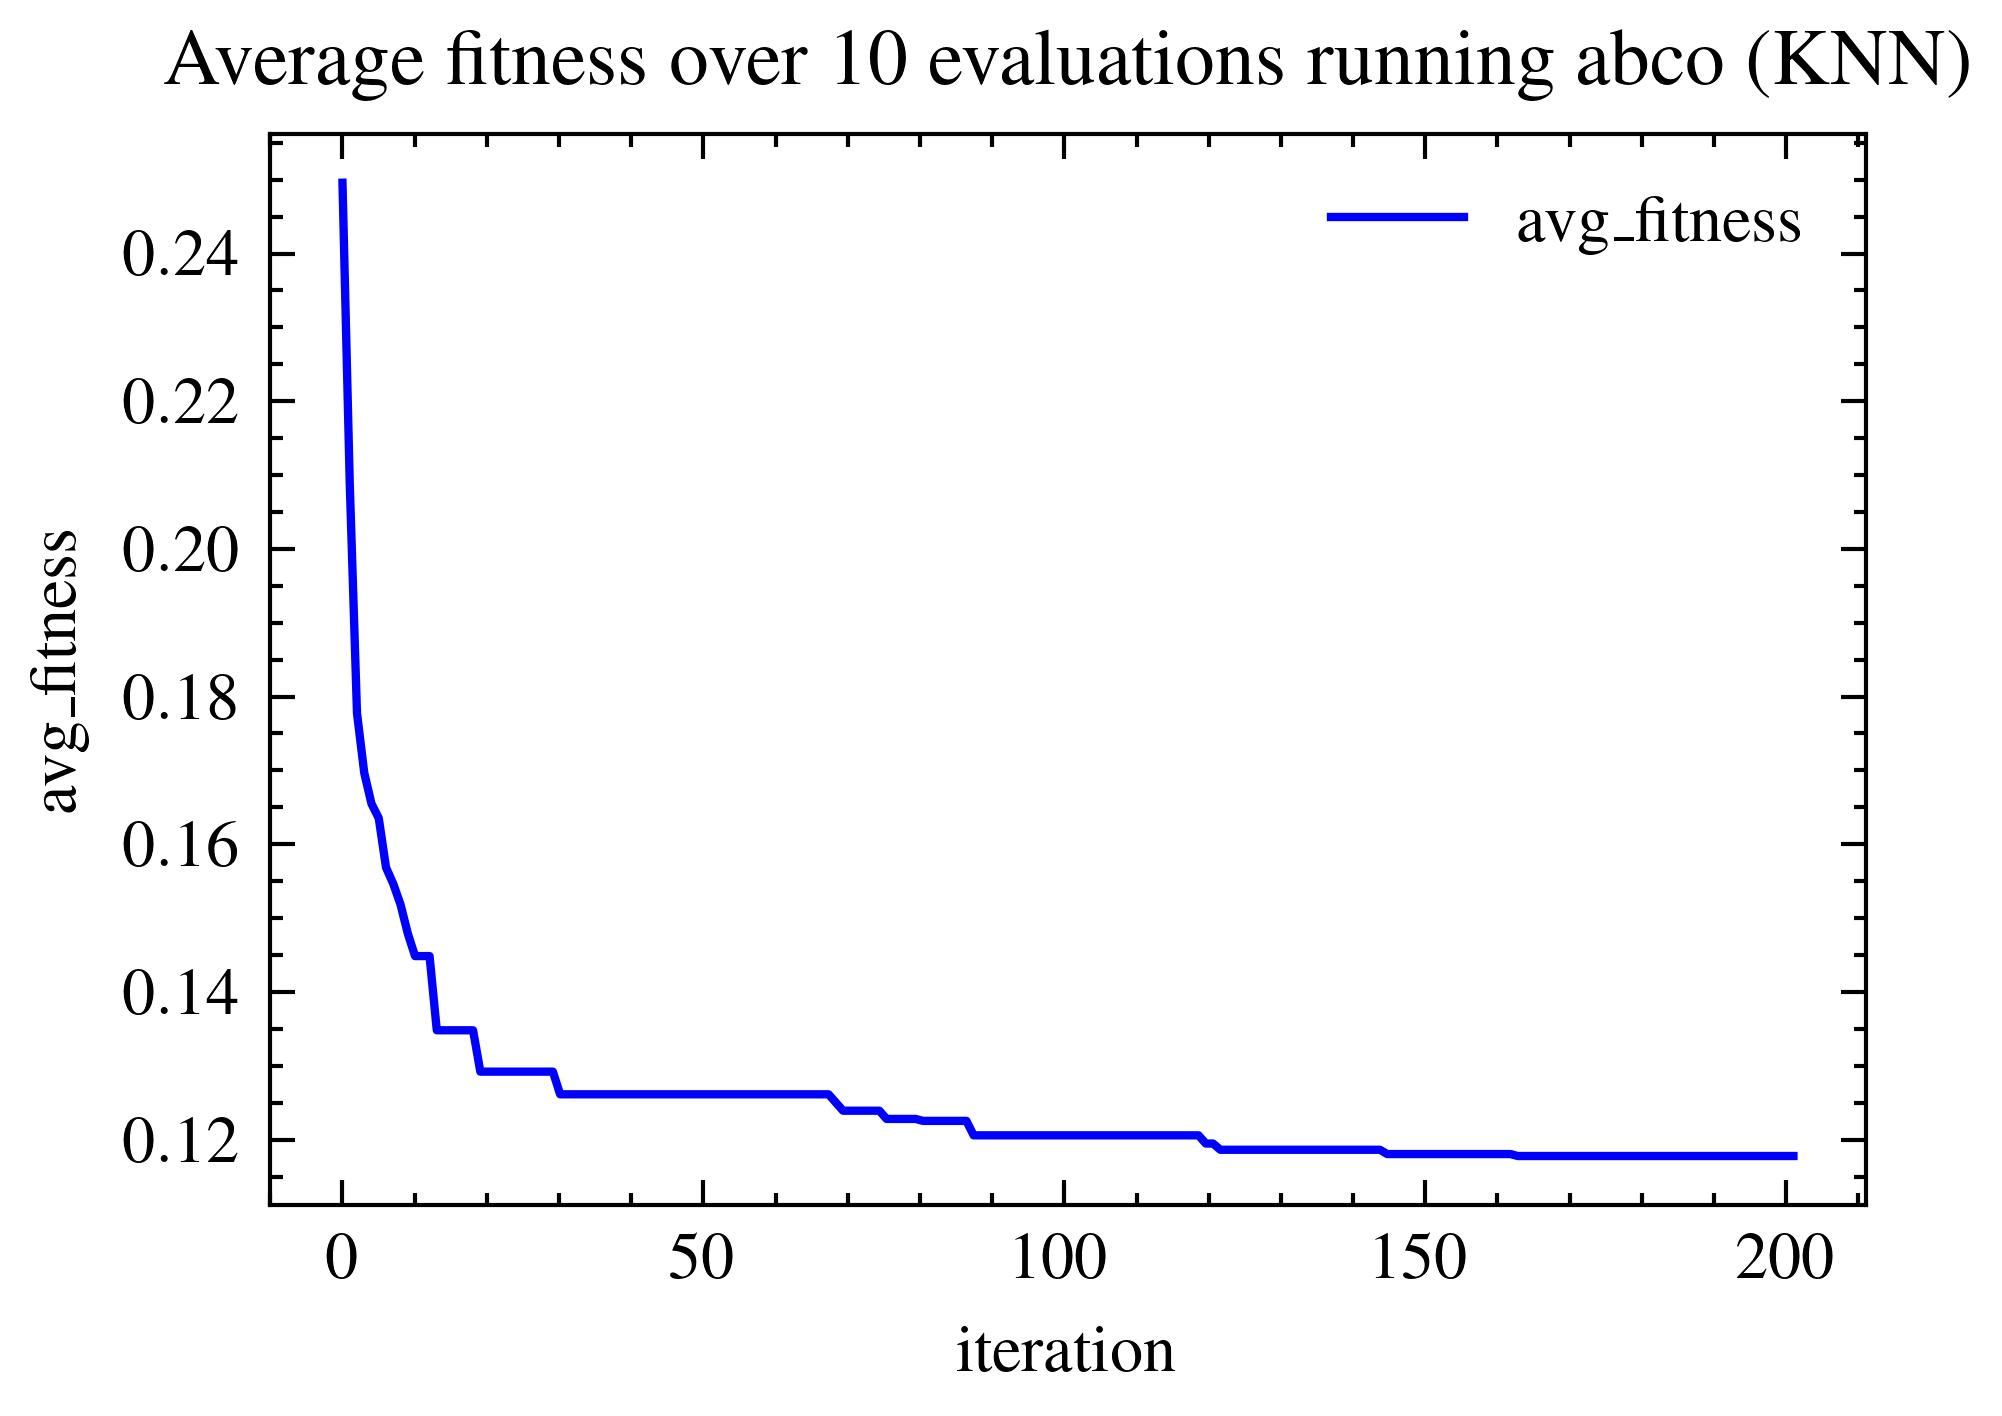
\includegraphics[width=\textwidth]{imagenes/binary_knn_fitness/KNN_fitness_over_10_evaluations_abco_binary_breast-cancer.jpg}
        \caption{ABCO}
        \label{fig:sub1}
    \end{subfigure}
    \hfill
    \begin{subfigure}[b]{0.3\textwidth}
        \centering
        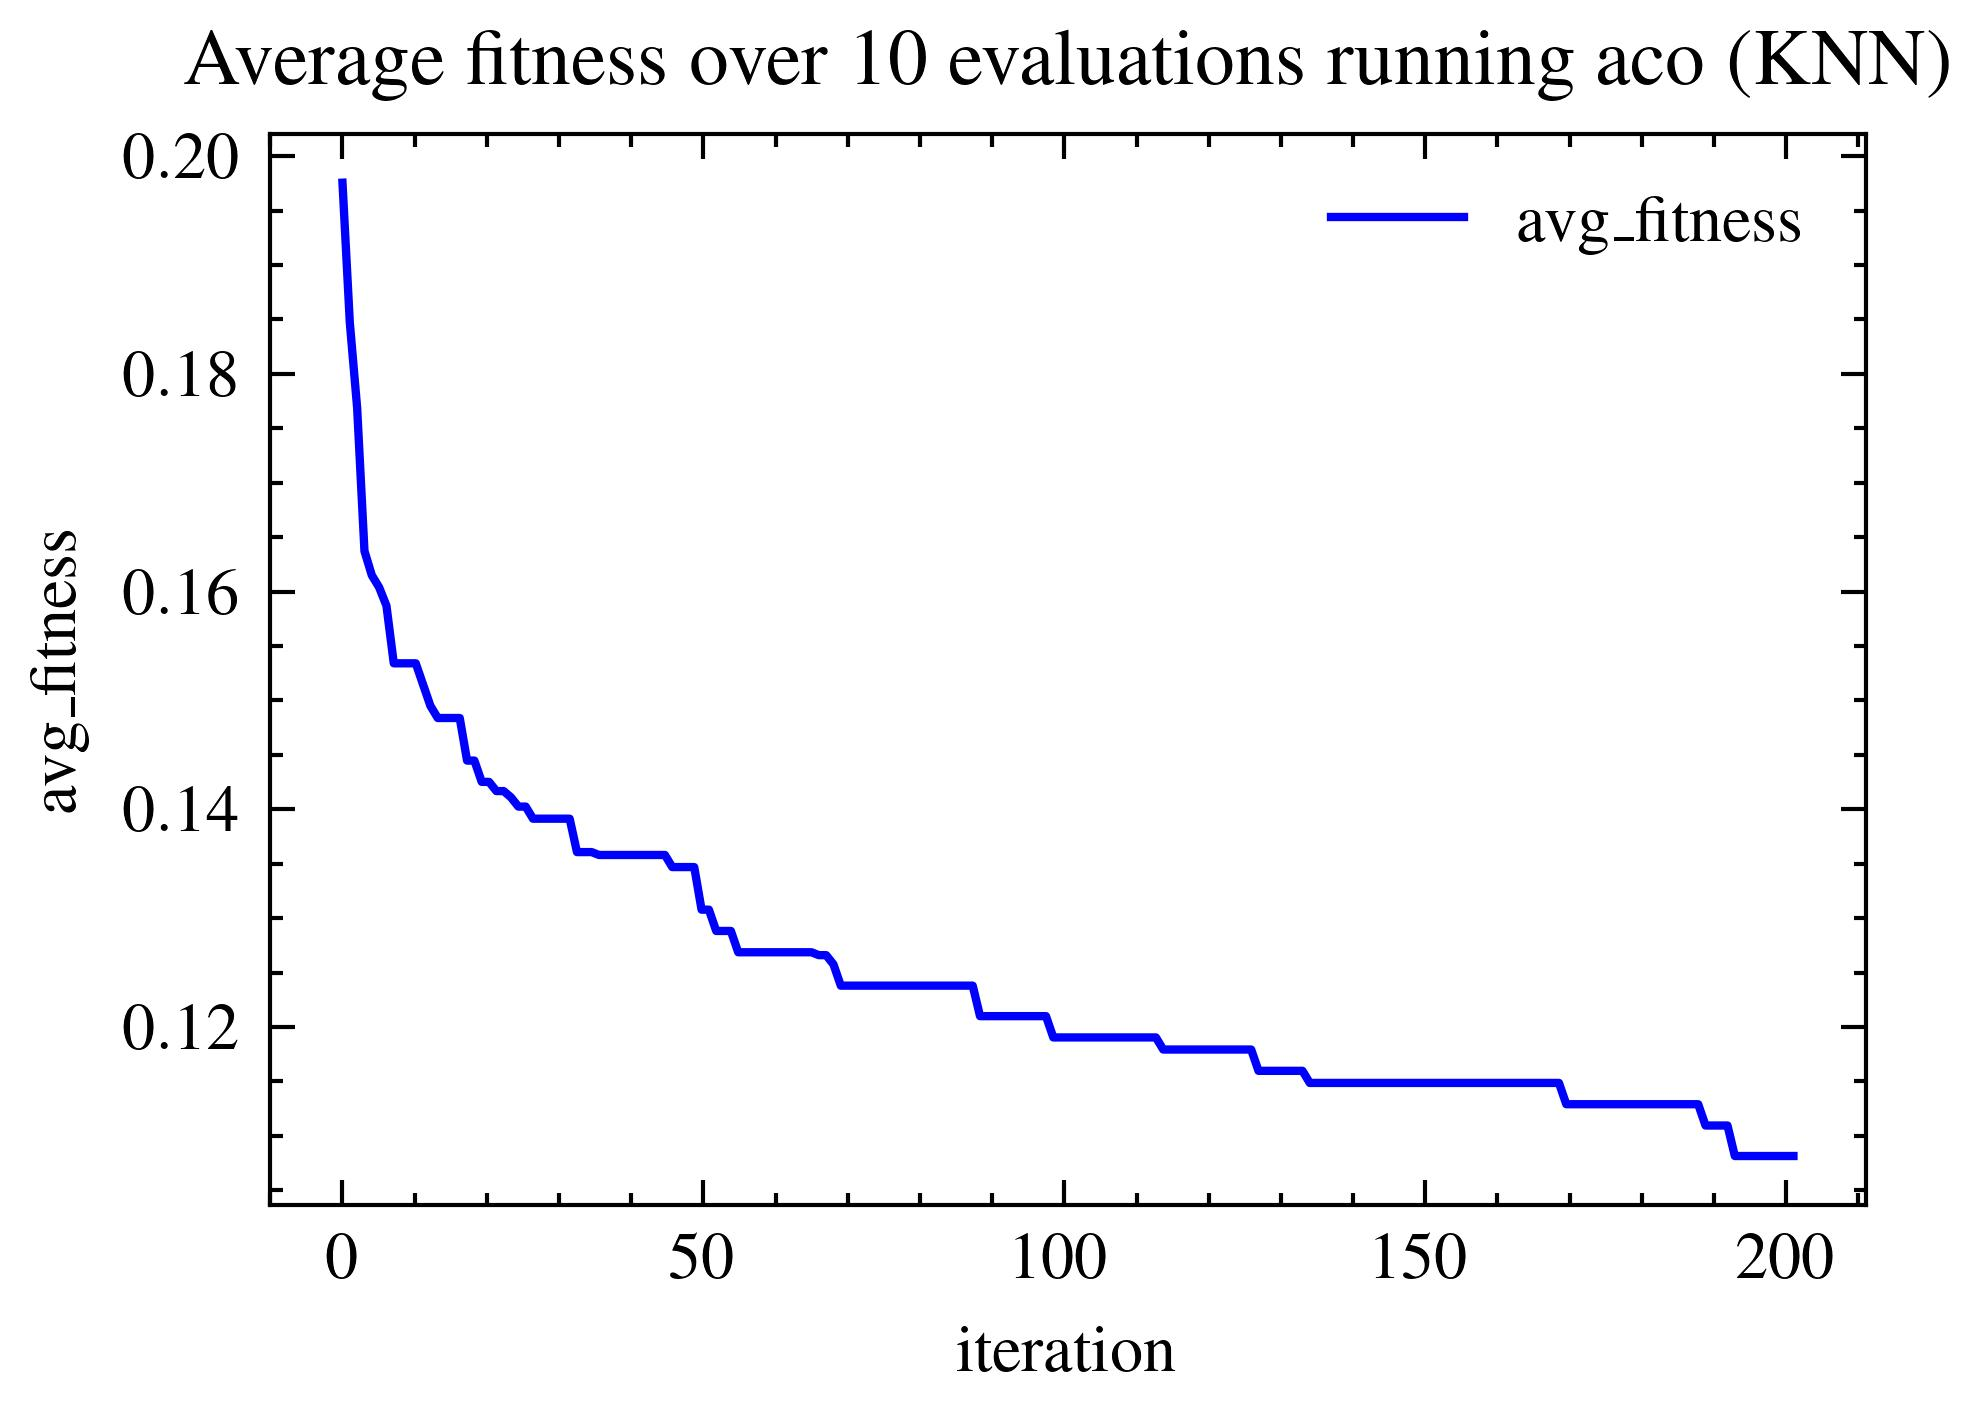
\includegraphics[width=\textwidth]{imagenes/binary_knn_fitness/KNN_fitness_over_10_evaluations_aco_binary_breast-cancer.jpg}
        \caption{ACO}
        \label{fig:sub2}
    \end{subfigure}
    \hfill
    \begin{subfigure}[b]{0.3\textwidth}
        \centering
        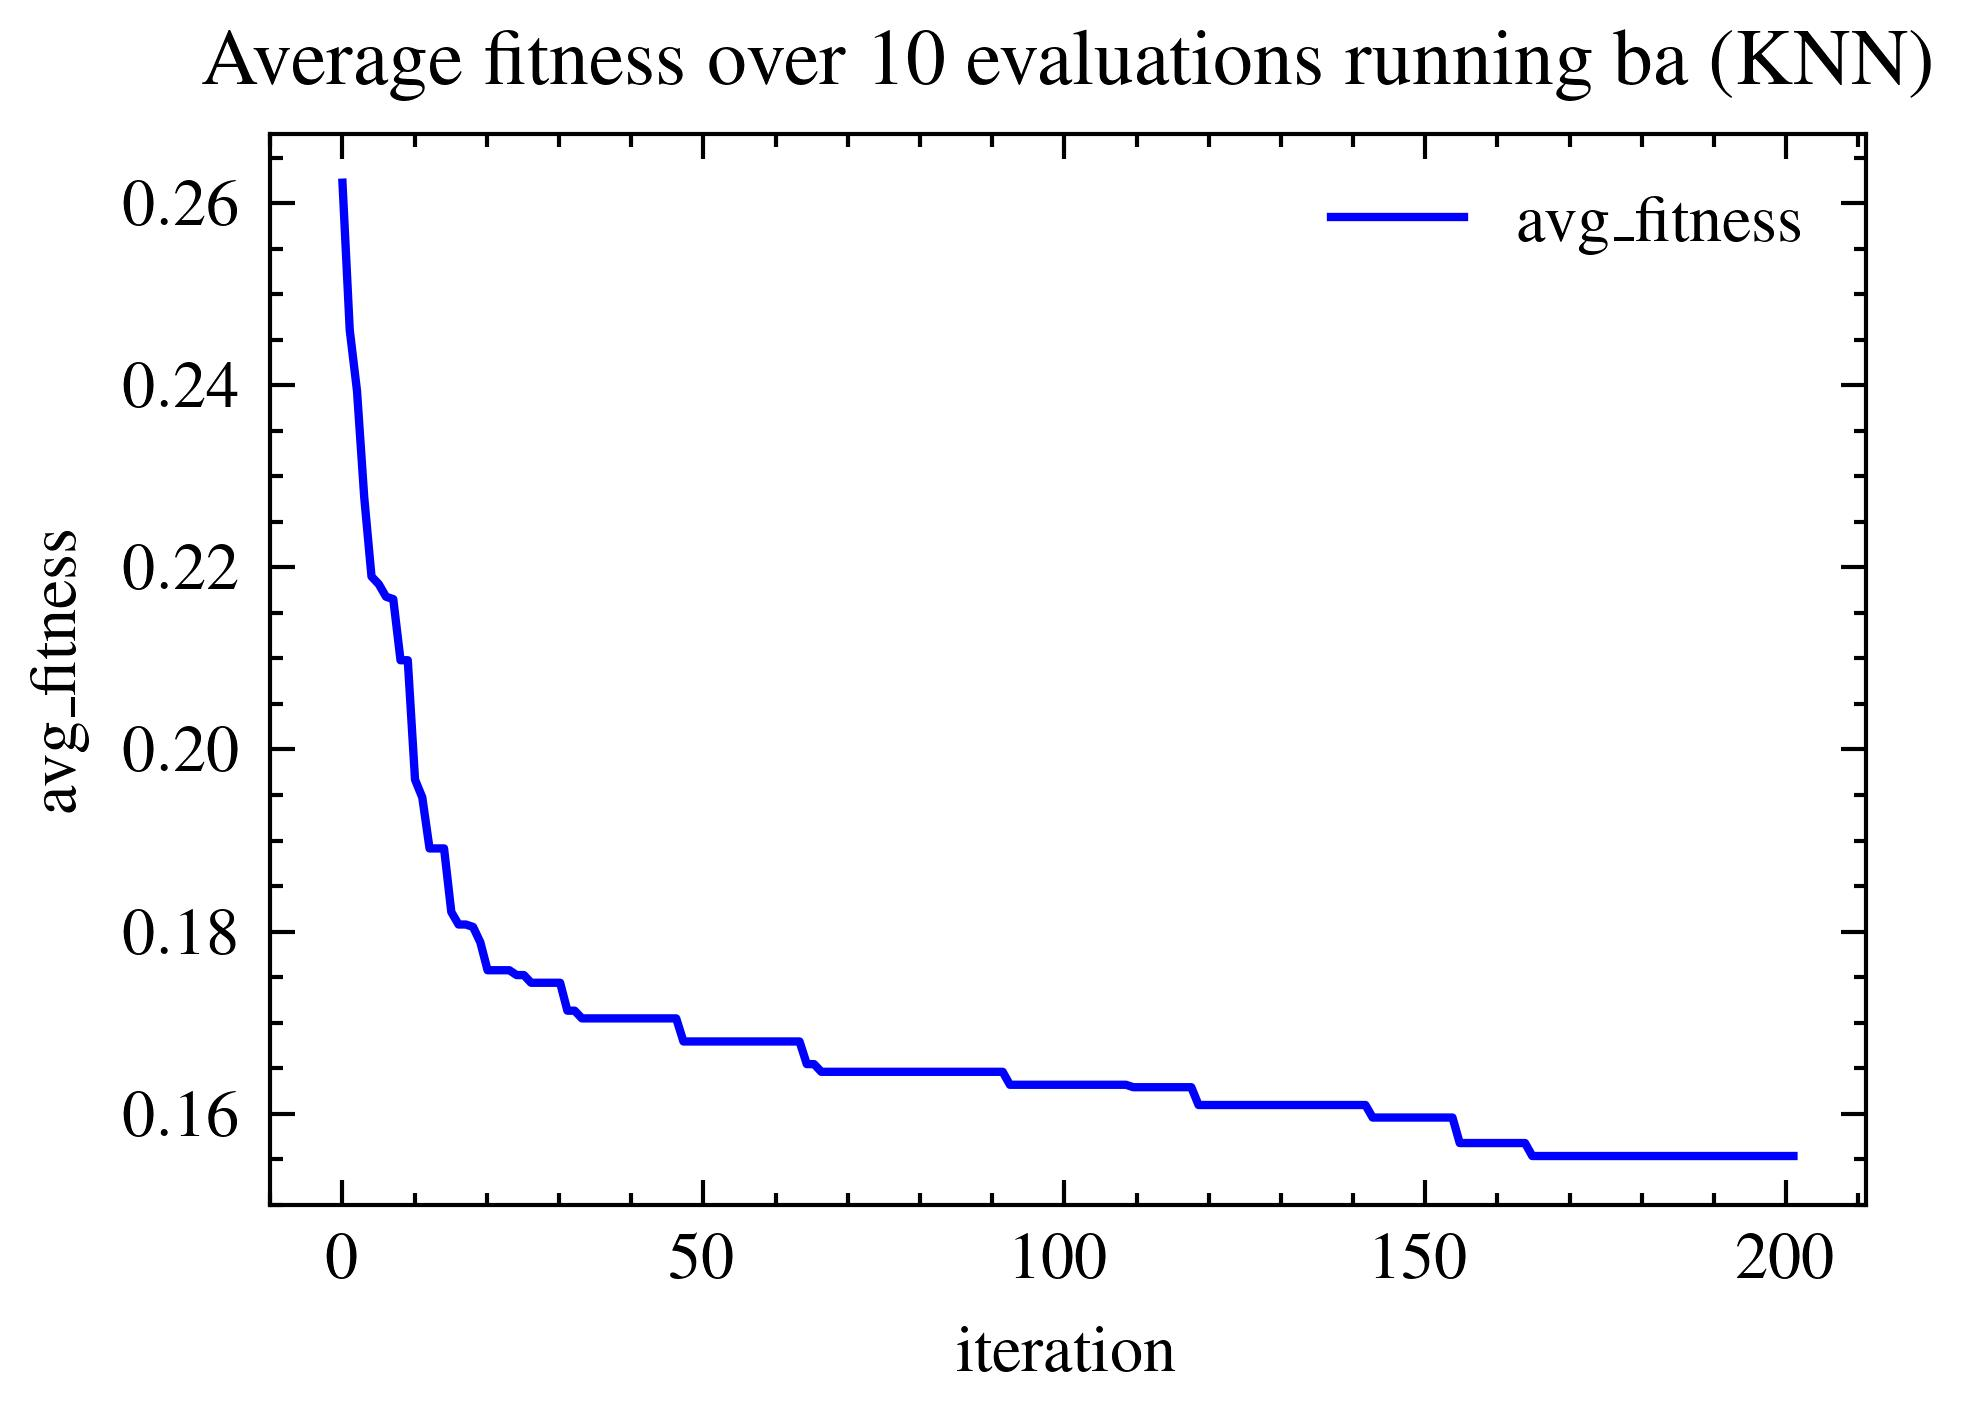
\includegraphics[width=\textwidth]{imagenes/binary_knn_fitness/KNN_fitness_over_10_evaluations_ba_binary_breast-cancer.jpg}
        \caption{BA}
        \label{fig:sub3}
    \end{subfigure}

    \begin{subfigure}[b]{0.3\textwidth}
        \centering
        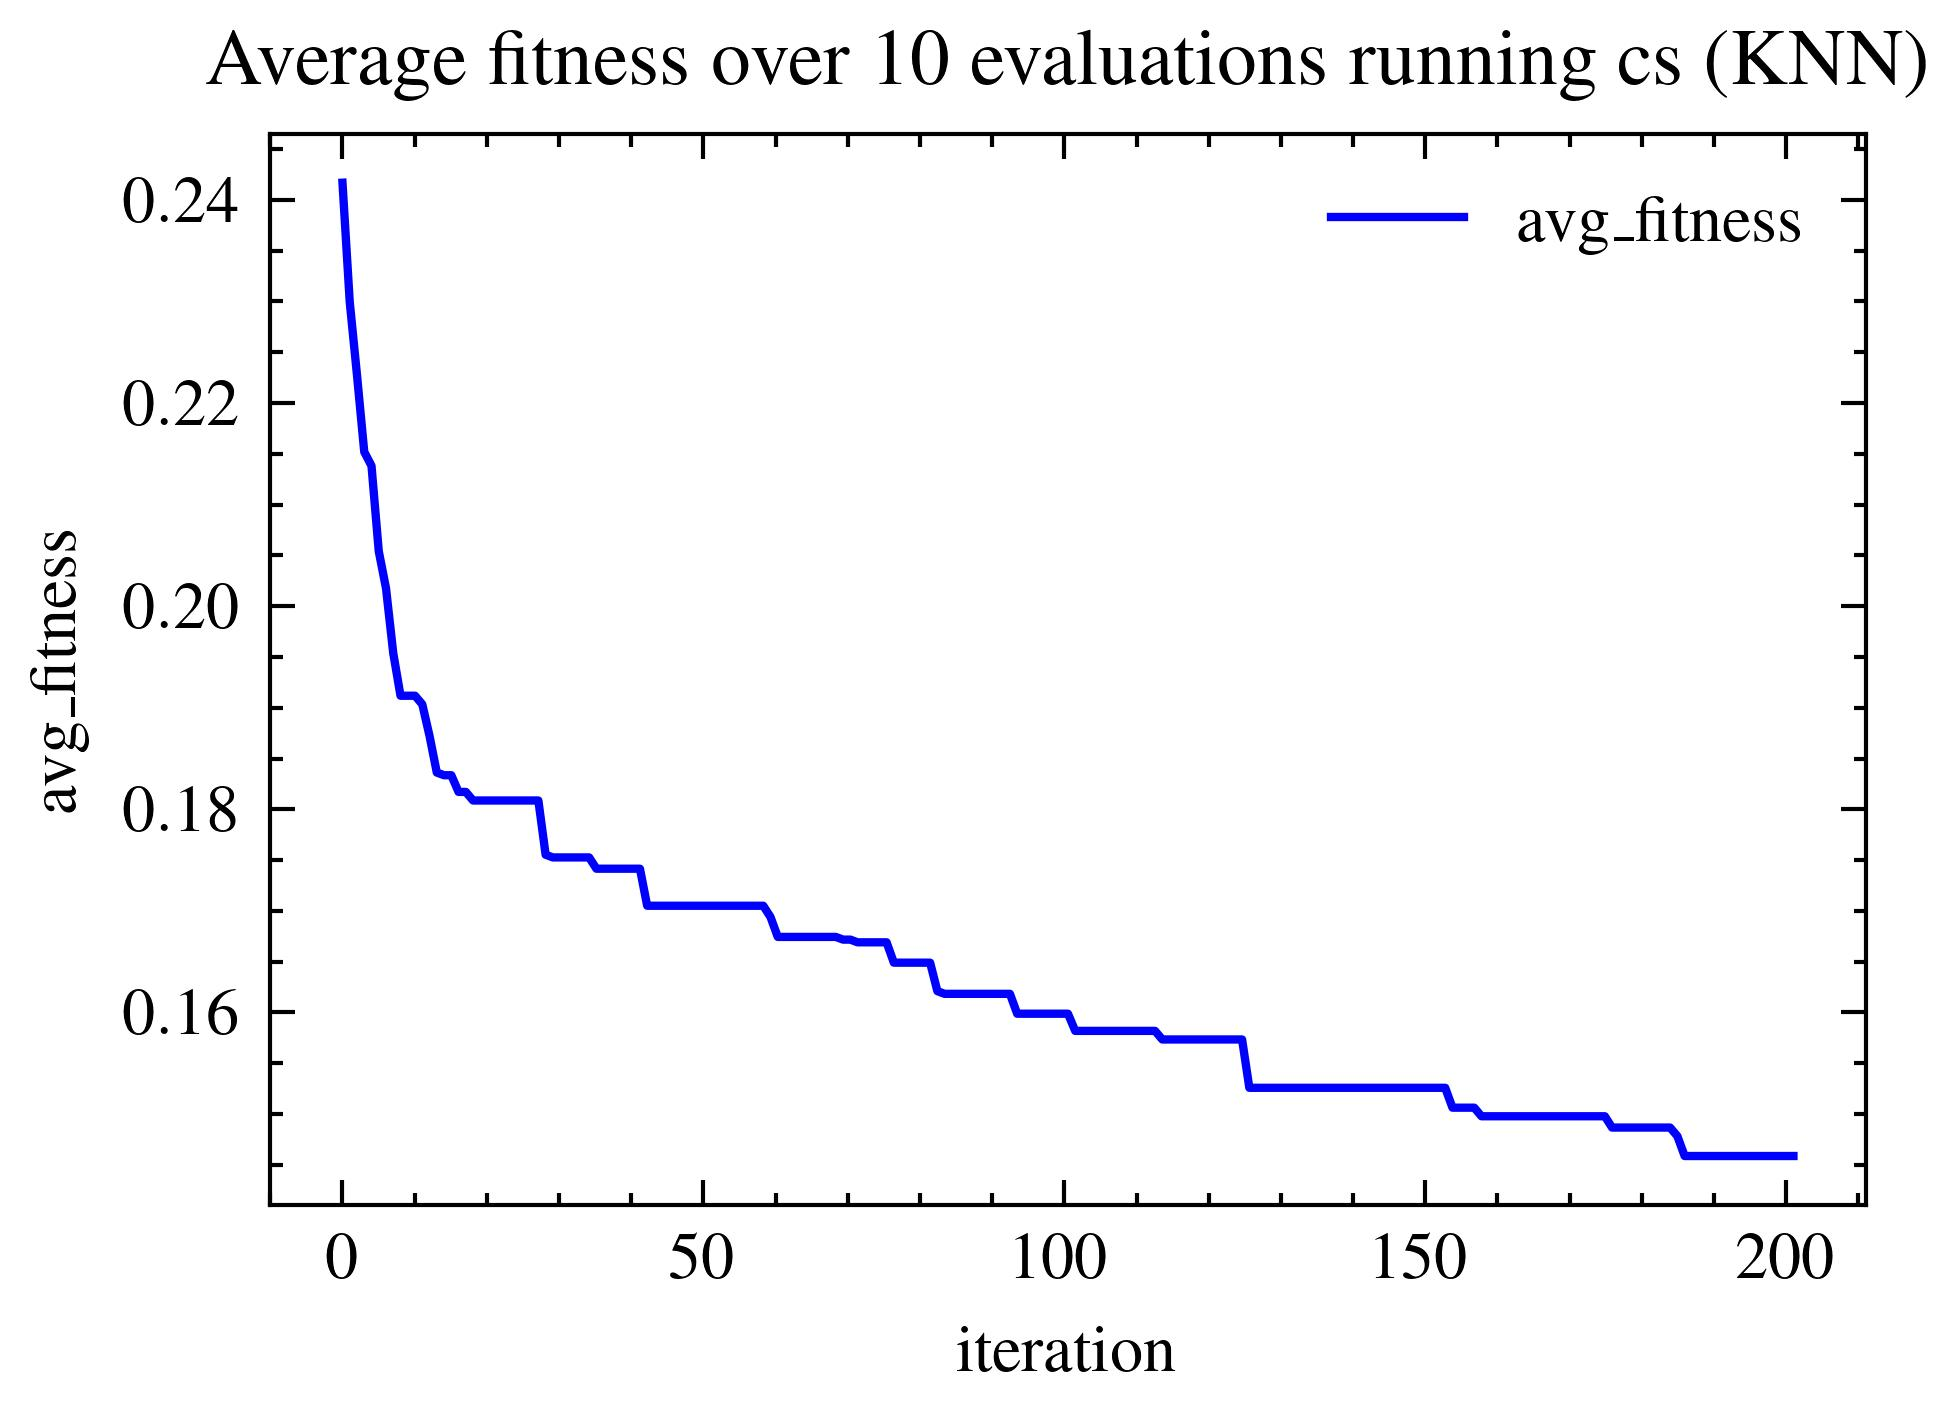
\includegraphics[width=\textwidth]{imagenes/binary_knn_fitness/KNN_fitness_over_10_evaluations_cs_binary_breast-cancer.jpg}
        \caption{CS}
        \label{fig:sub4}
    \end{subfigure}
    \hfill
    \begin{subfigure}[b]{0.3\textwidth}
        \centering
        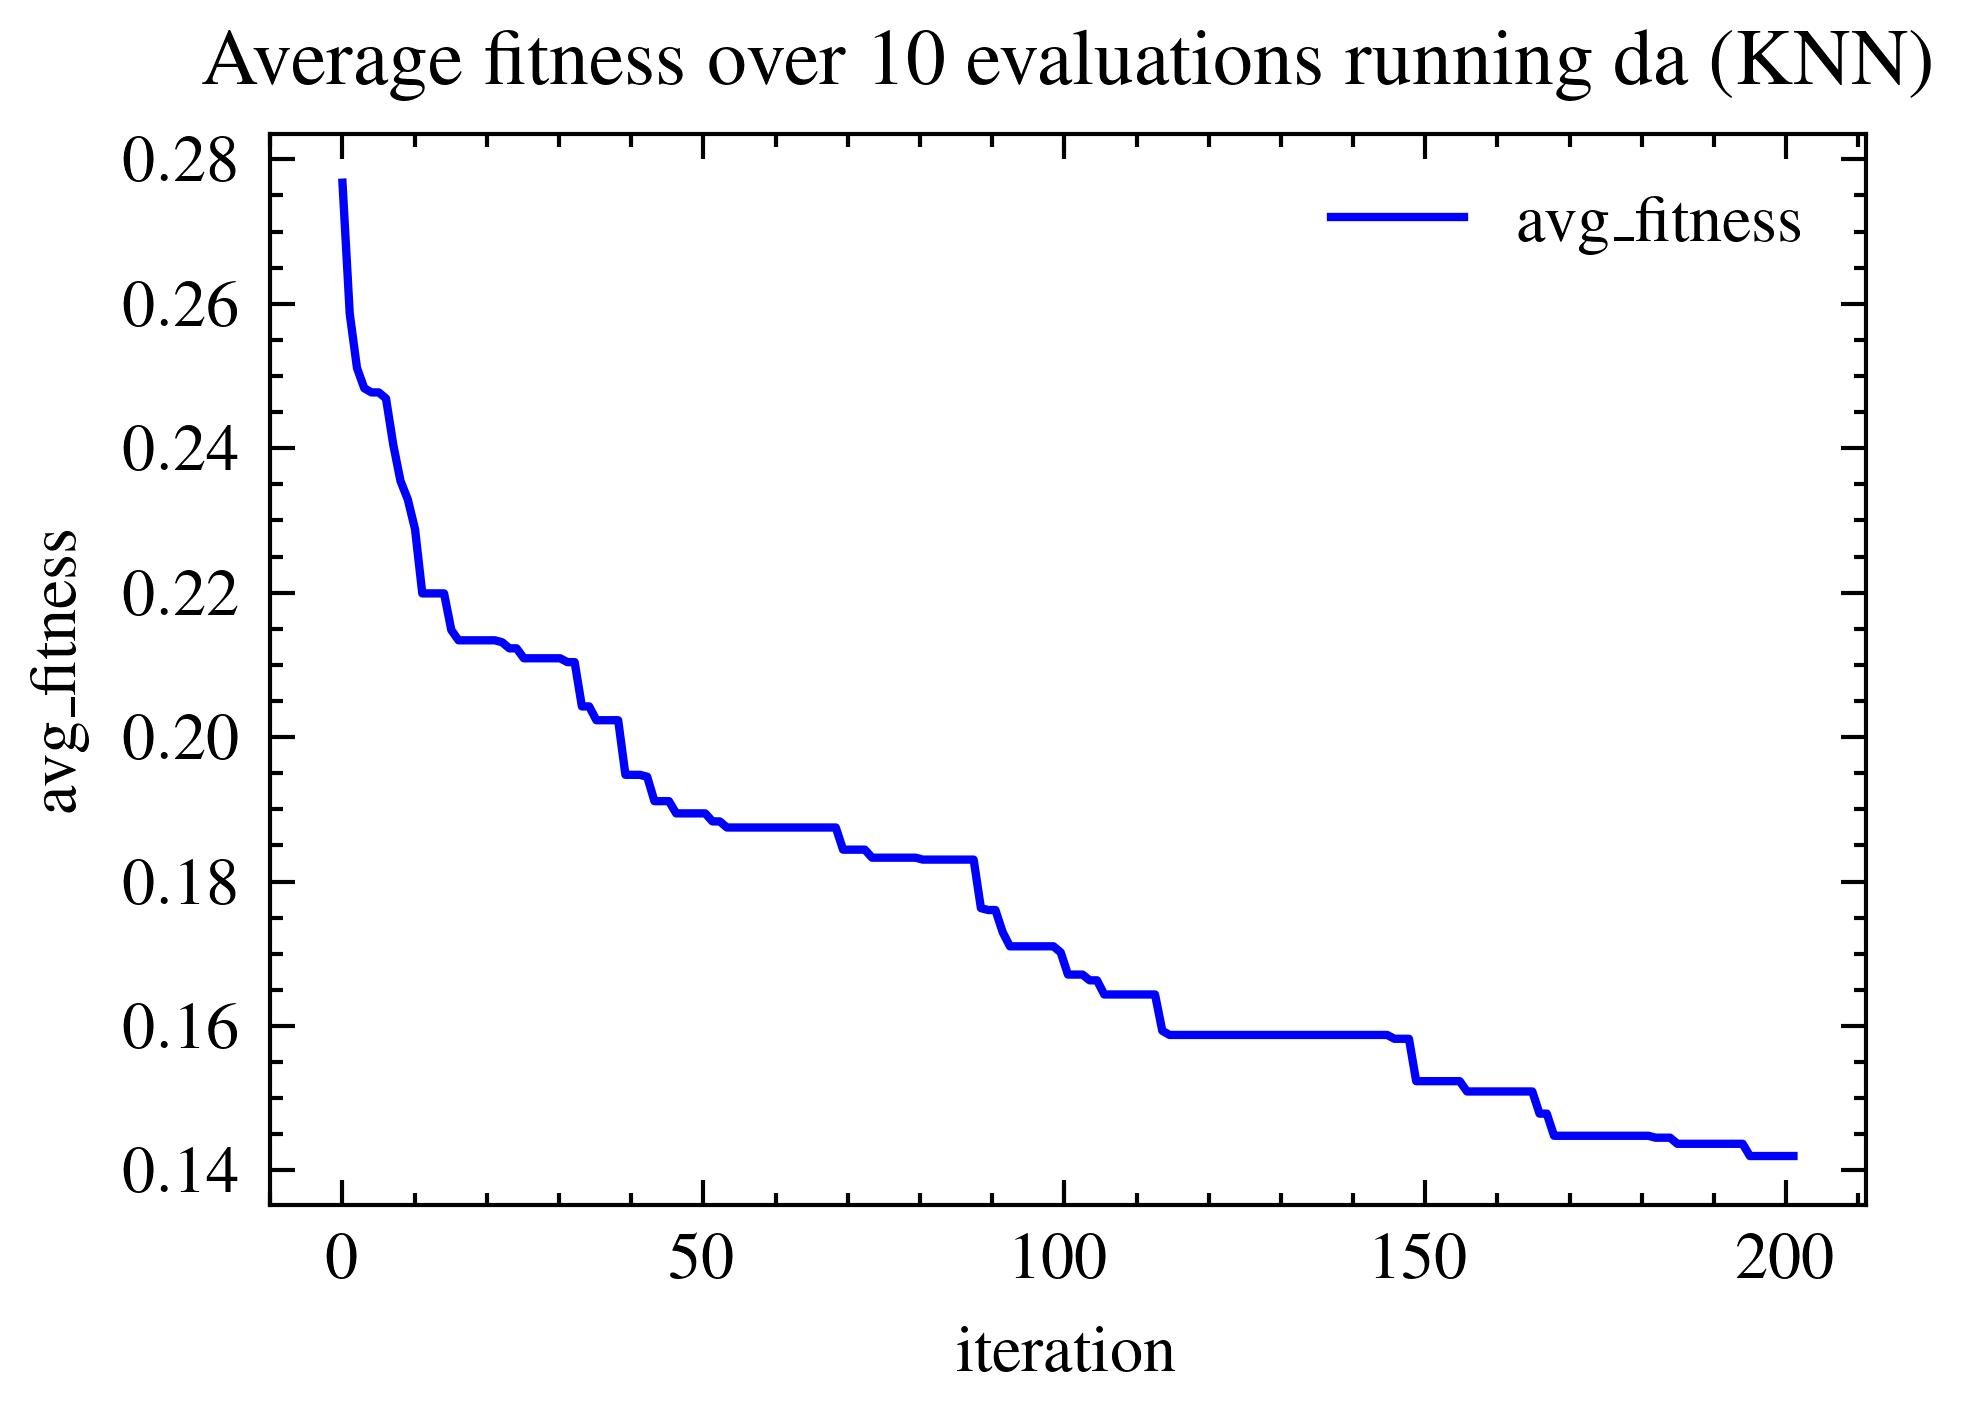
\includegraphics[width=\textwidth]{imagenes/binary_knn_fitness/KNN_fitness_over_10_evaluations_da_binary_breast-cancer.jpg}
        \caption{DA}
        \label{fig:sub5}
    \end{subfigure}
    \hfill
    \begin{subfigure}[b]{0.3\textwidth}
        \centering
        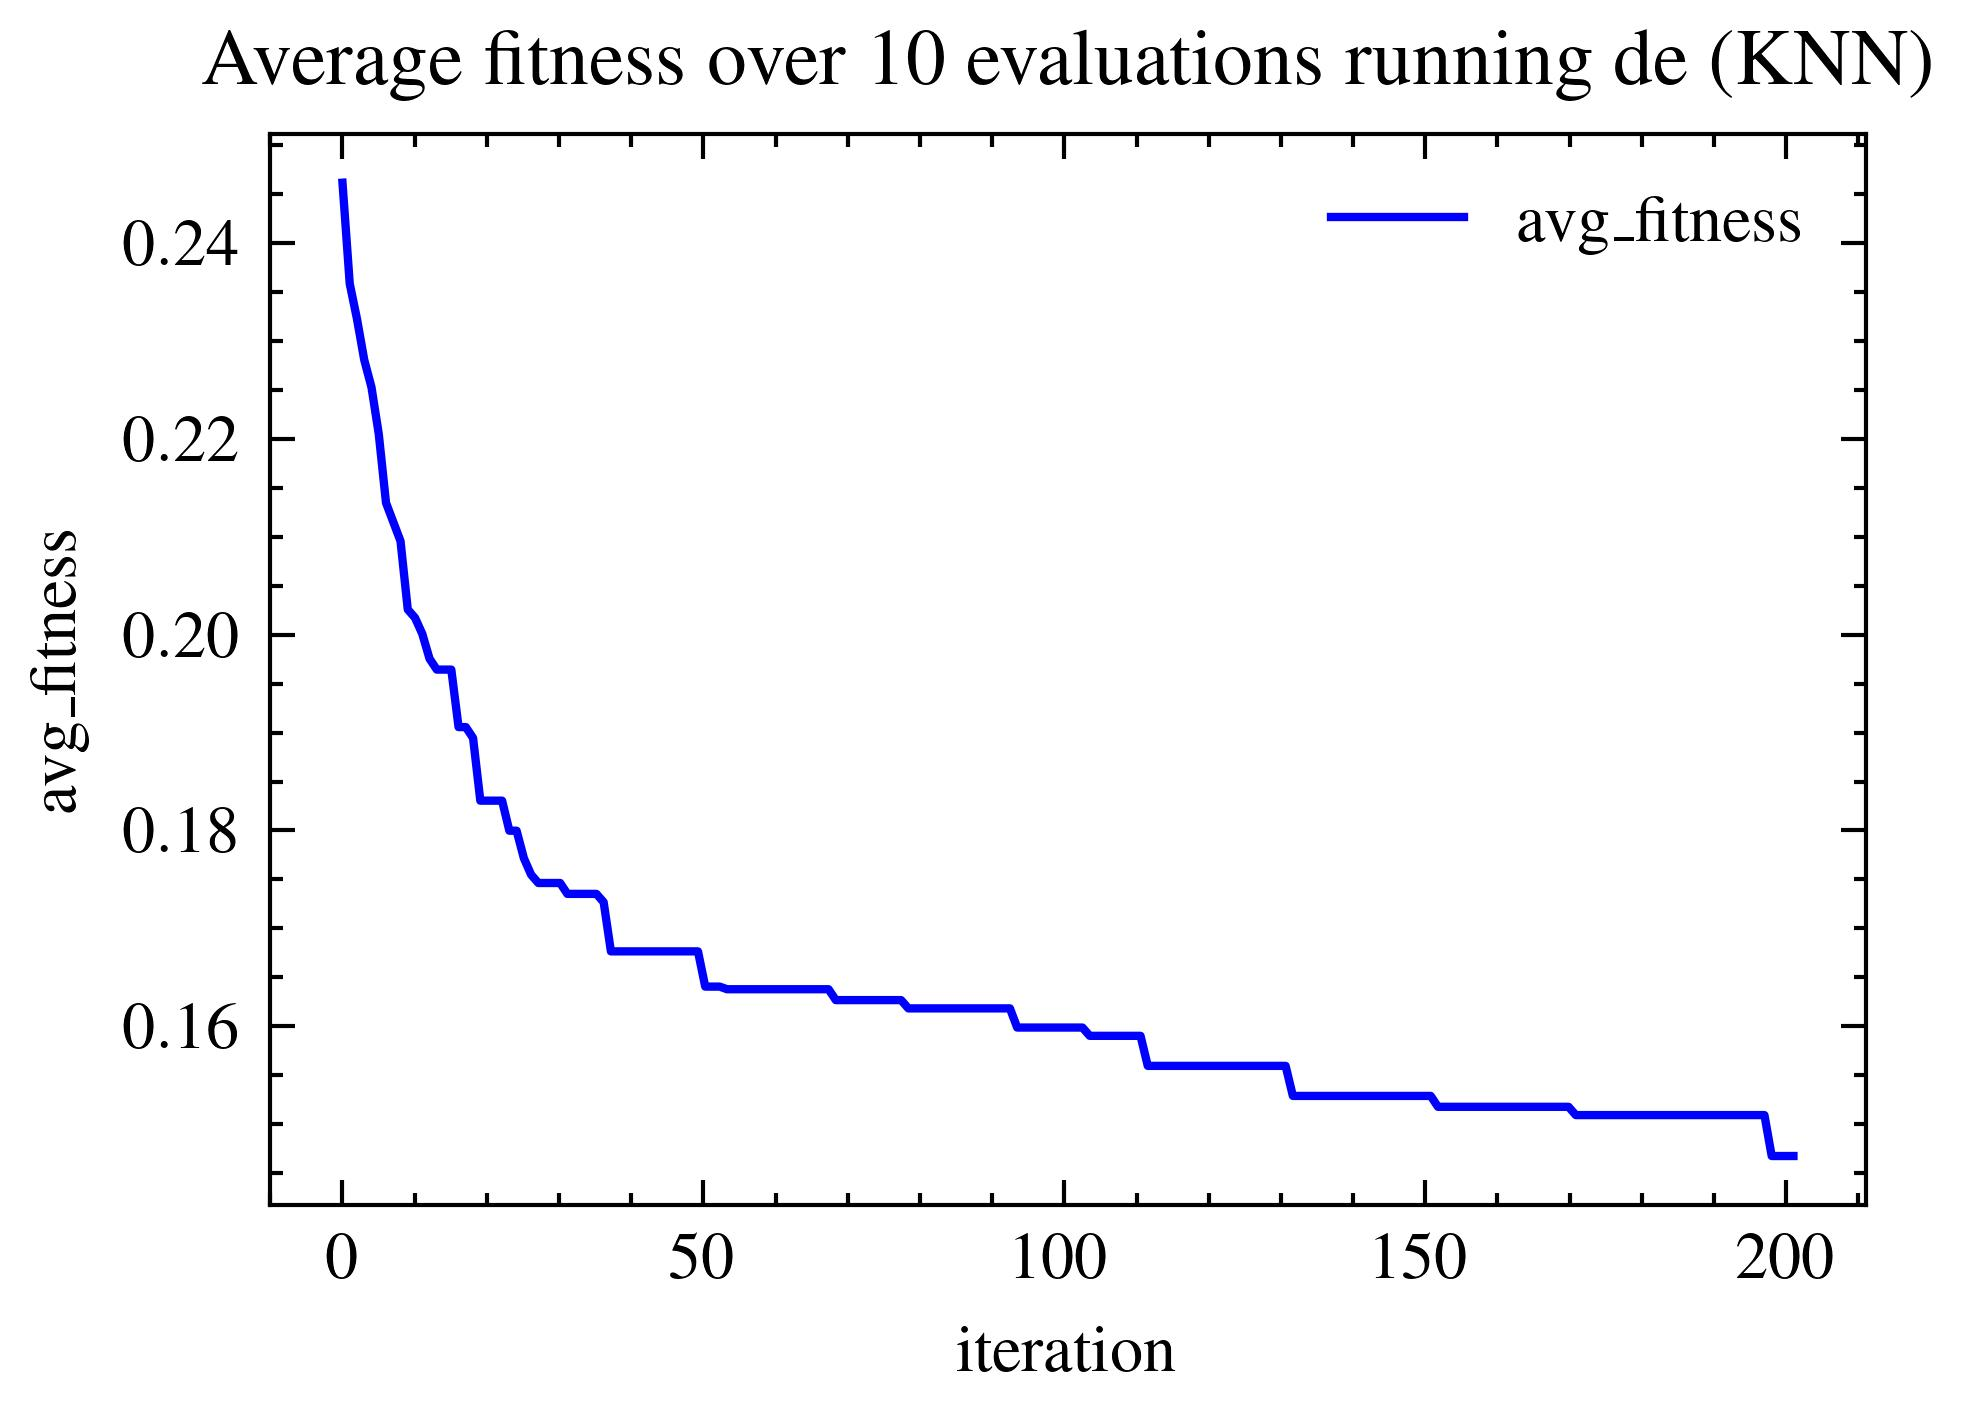
\includegraphics[width=\textwidth]{imagenes/binary_knn_fitness/KNN_fitness_over_10_evaluations_de_binary_breast-cancer.jpg}
        \caption{DE}
        \label{fig:sub6}
    \end{subfigure}

    \begin{subfigure}[b]{0.3\textwidth}
        \centering
        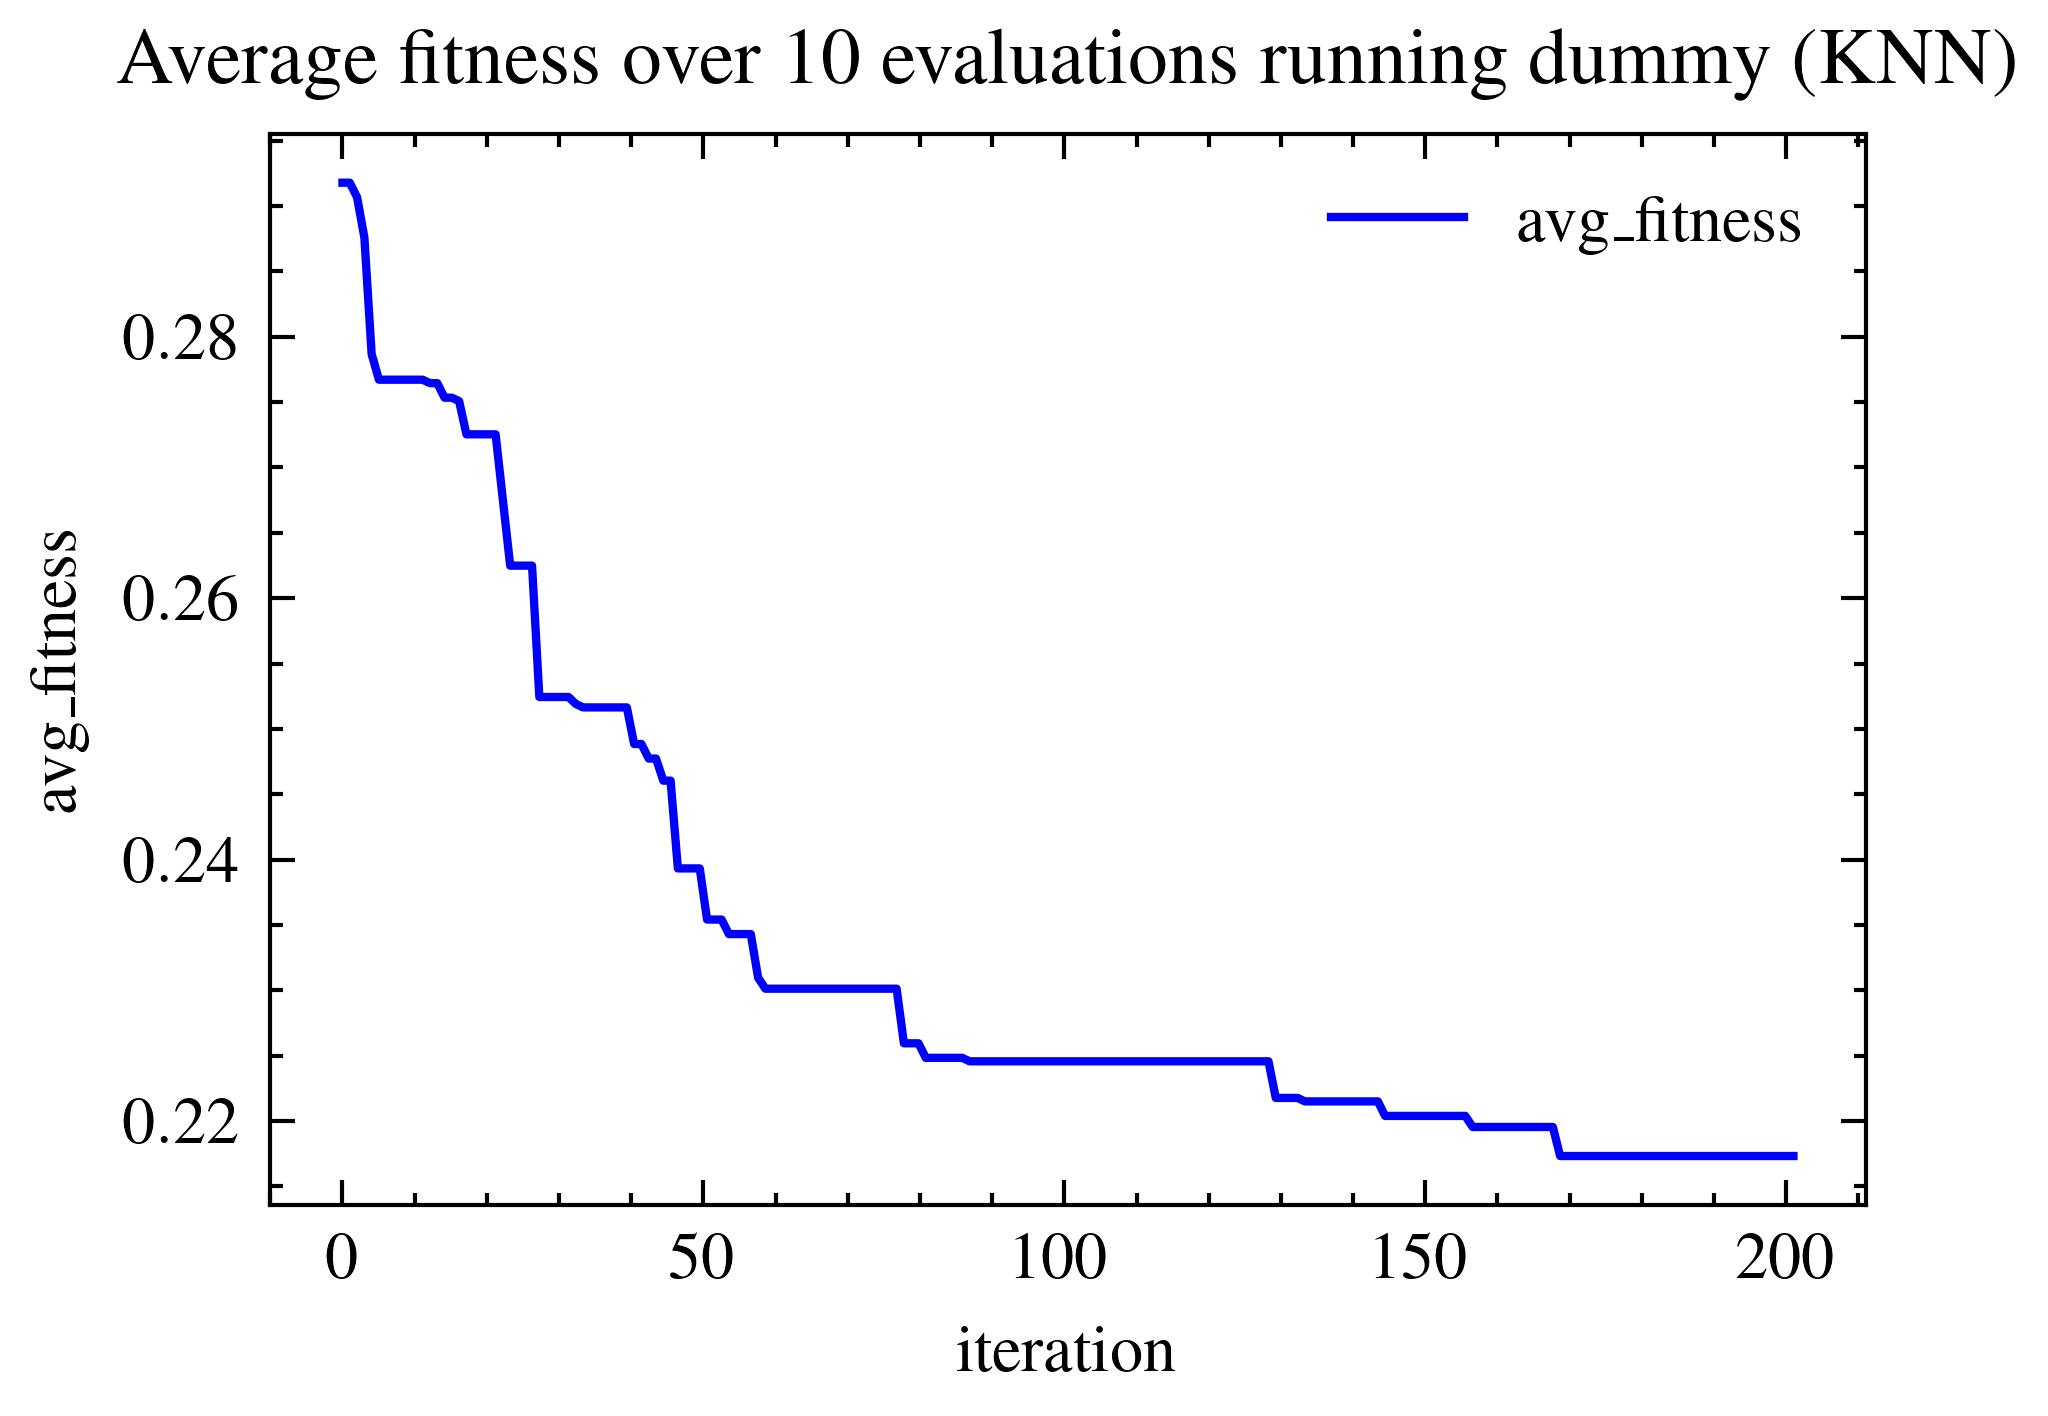
\includegraphics[width=\textwidth]{imagenes/binary_knn_fitness/KNN_fitness_over_10_evaluations_dummy_binary_breast-cancer.jpg}
        \caption{Dummy}
        \label{fig:sub7}
    \end{subfigure}
    \hfill
    \begin{subfigure}[b]{0.3\textwidth}
        \centering
        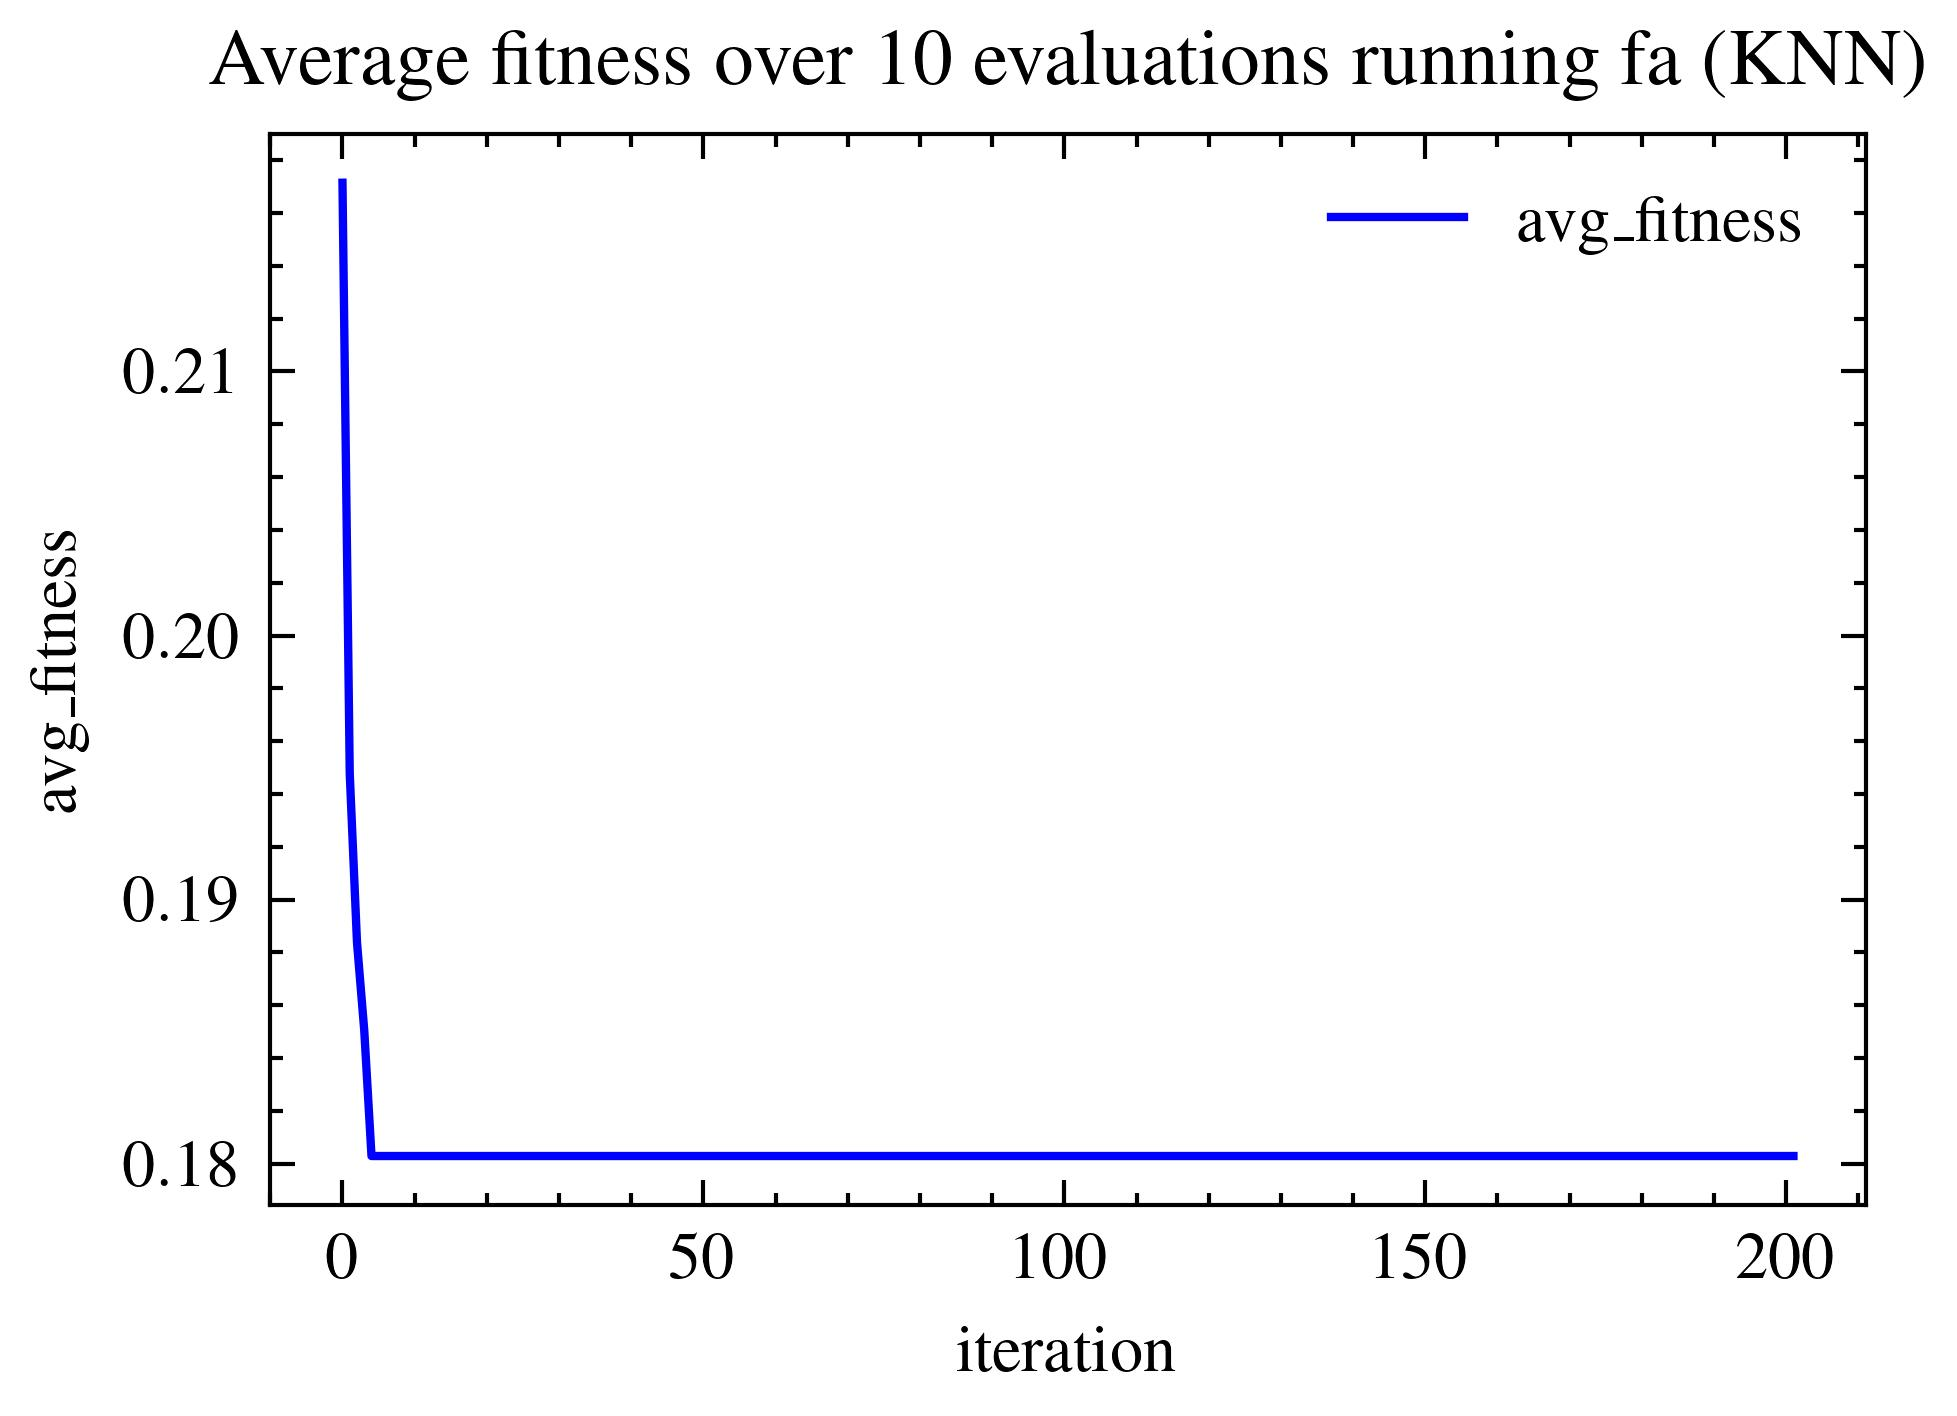
\includegraphics[width=\textwidth]{imagenes/binary_knn_fitness/KNN_fitness_over_10_evaluations_fa_binary_breast-cancer.jpg}
        \caption{FA}
        \label{fig:sub8}
    \end{subfigure}
    \hfill
    \begin{subfigure}[b]{0.3\textwidth}
        \centering
        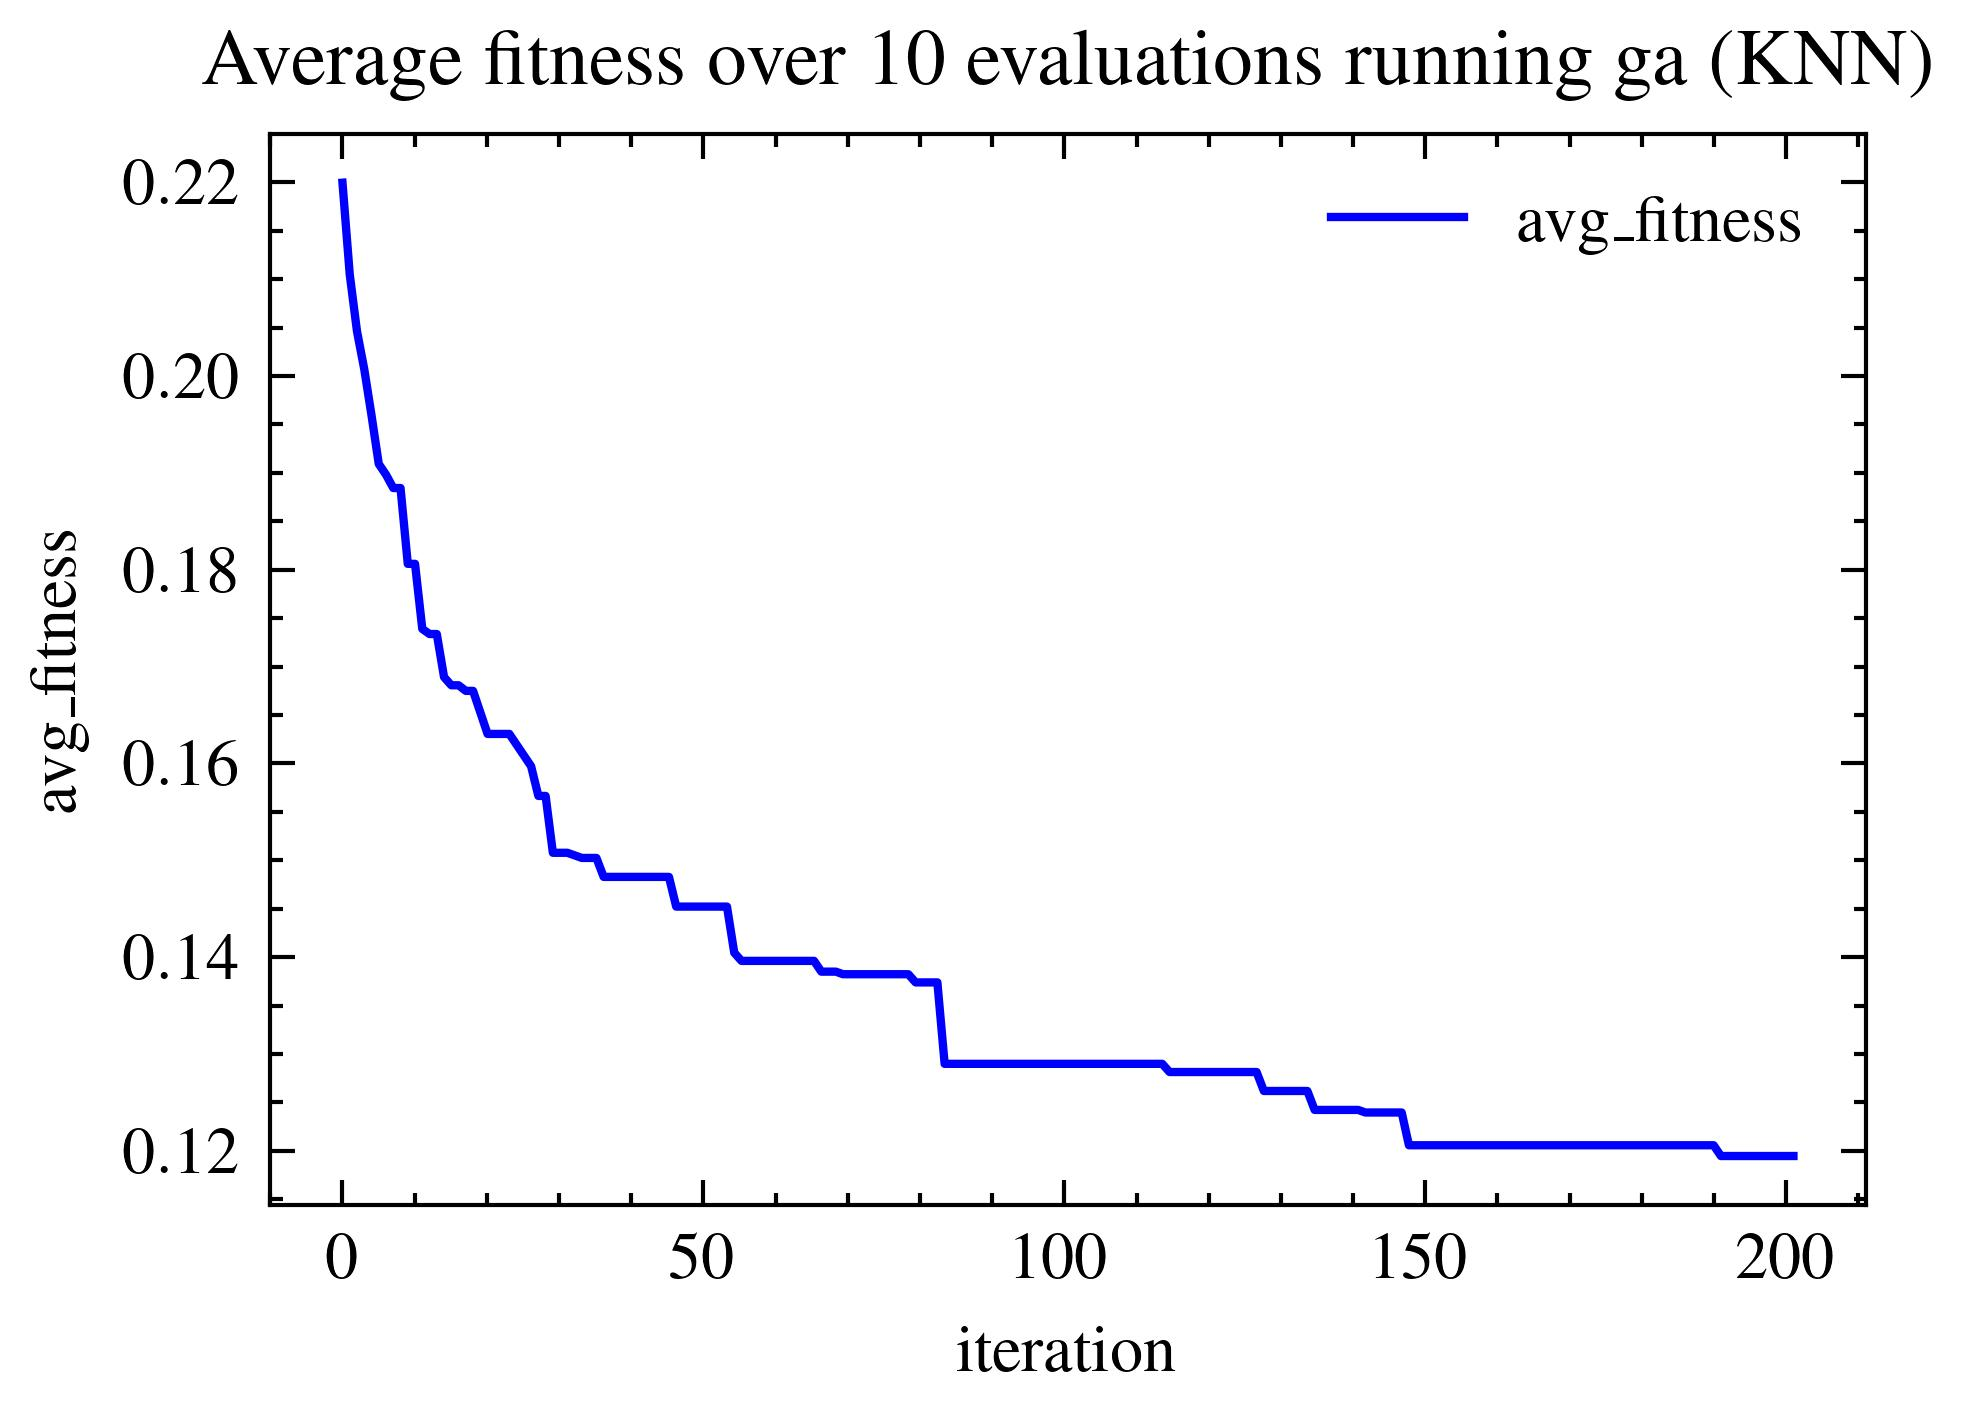
\includegraphics[width=\textwidth]{imagenes/binary_knn_fitness/KNN_fitness_over_10_evaluations_ga_binary_breast-cancer.jpg}
        \caption{GA}
        \label{fig:sub9}
    \end{subfigure}

    \begin{subfigure}[b]{0.3\textwidth}
        \centering
        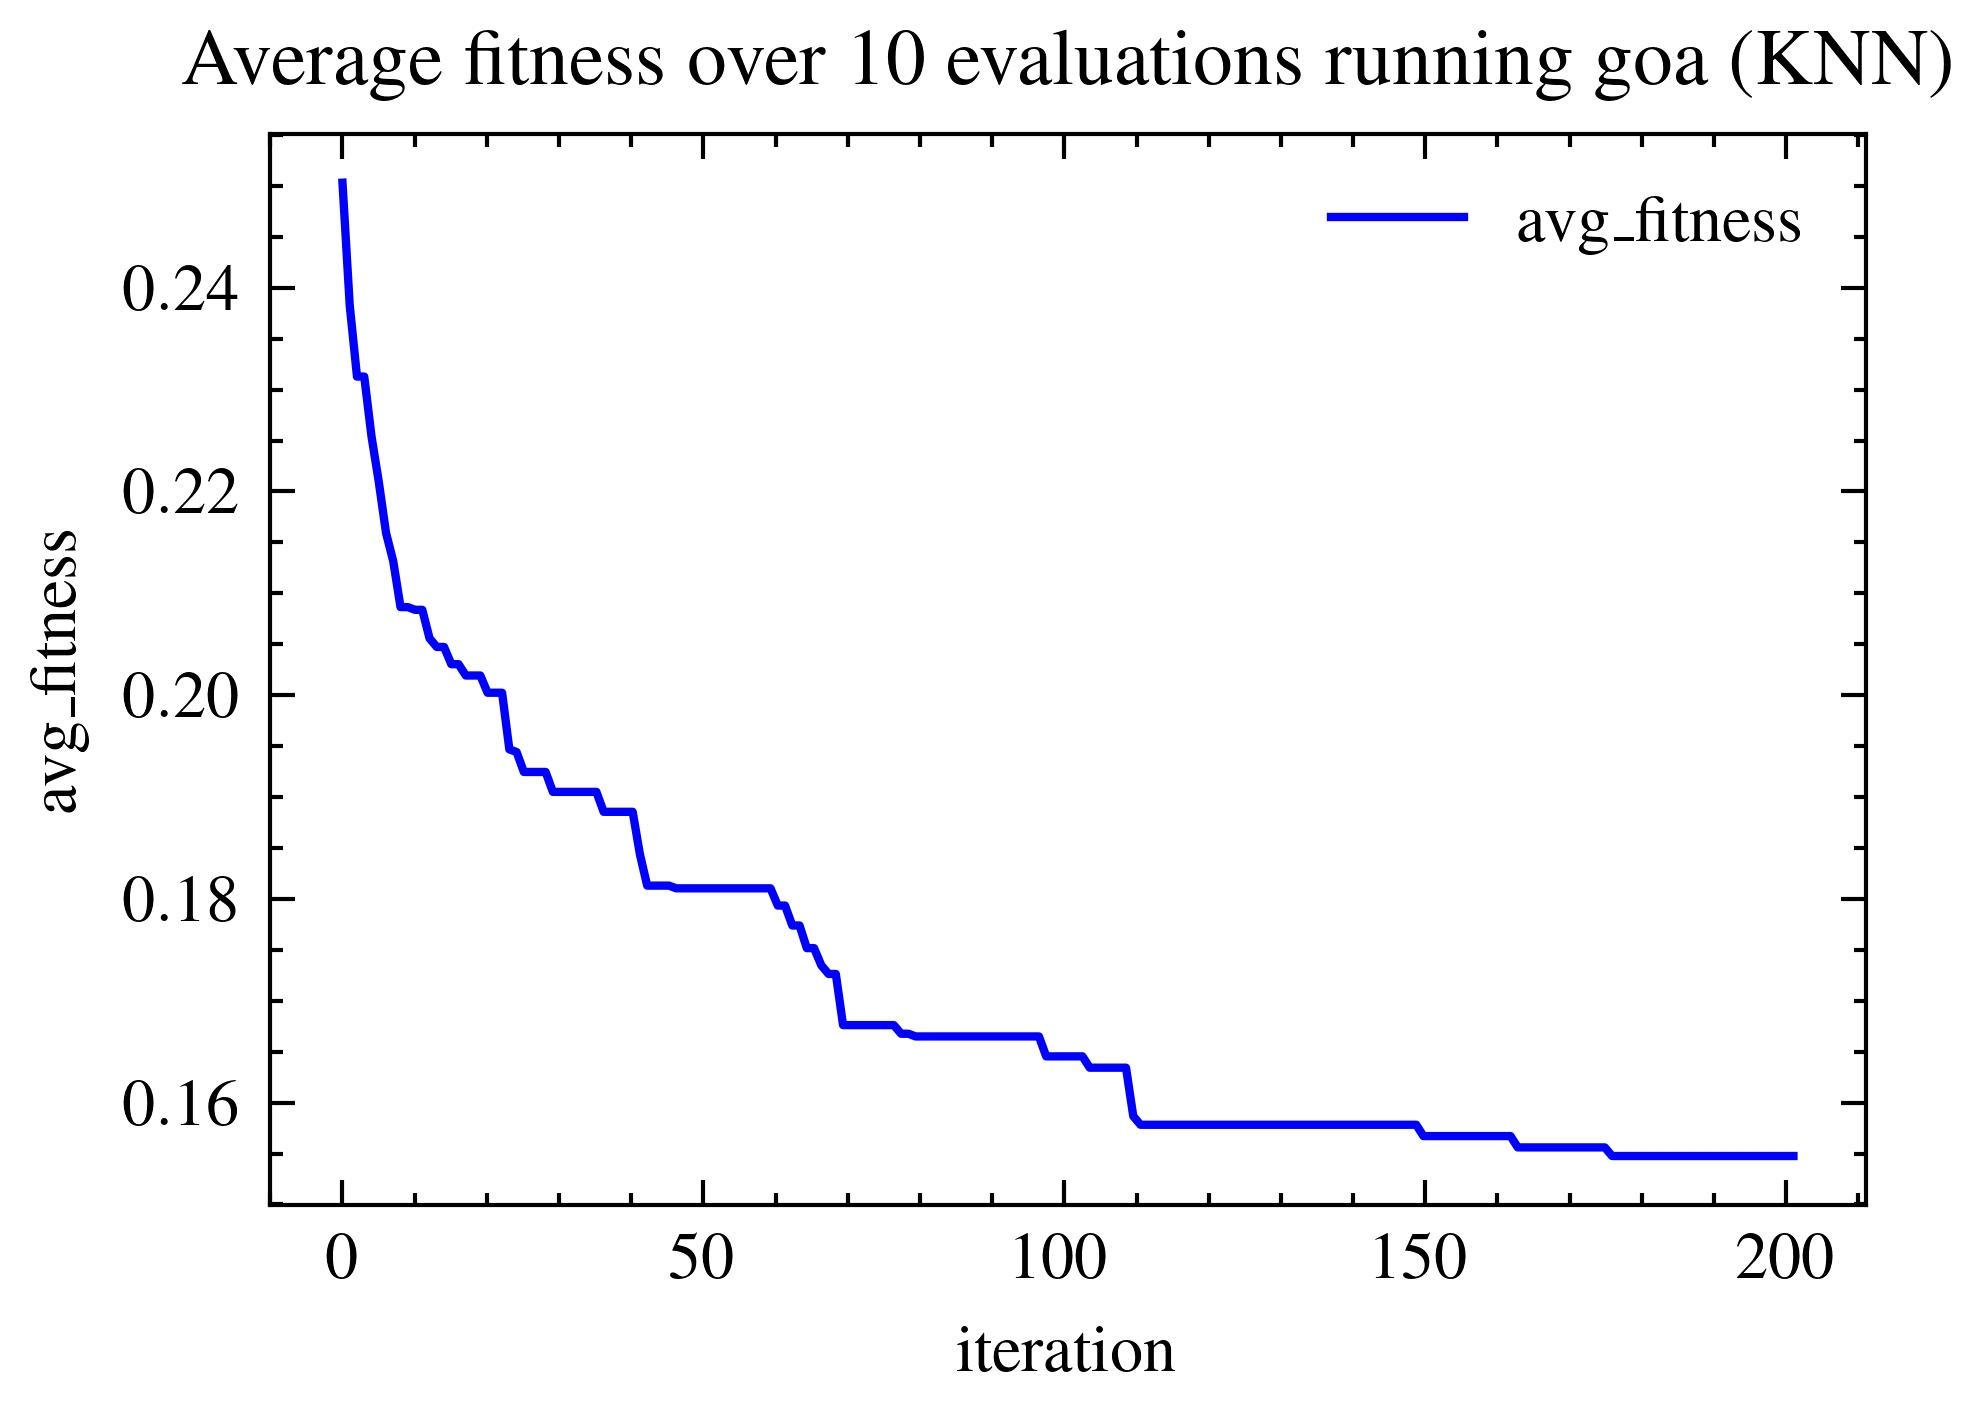
\includegraphics[width=\textwidth]{imagenes/binary_knn_fitness/KNN_fitness_over_10_evaluations_goa_binary_breast-cancer.jpg}
        \caption{GOA}
        \label{fig:sub10}
    \end{subfigure}
    \hfill
    \begin{subfigure}[b]{0.3\textwidth}
        \centering
        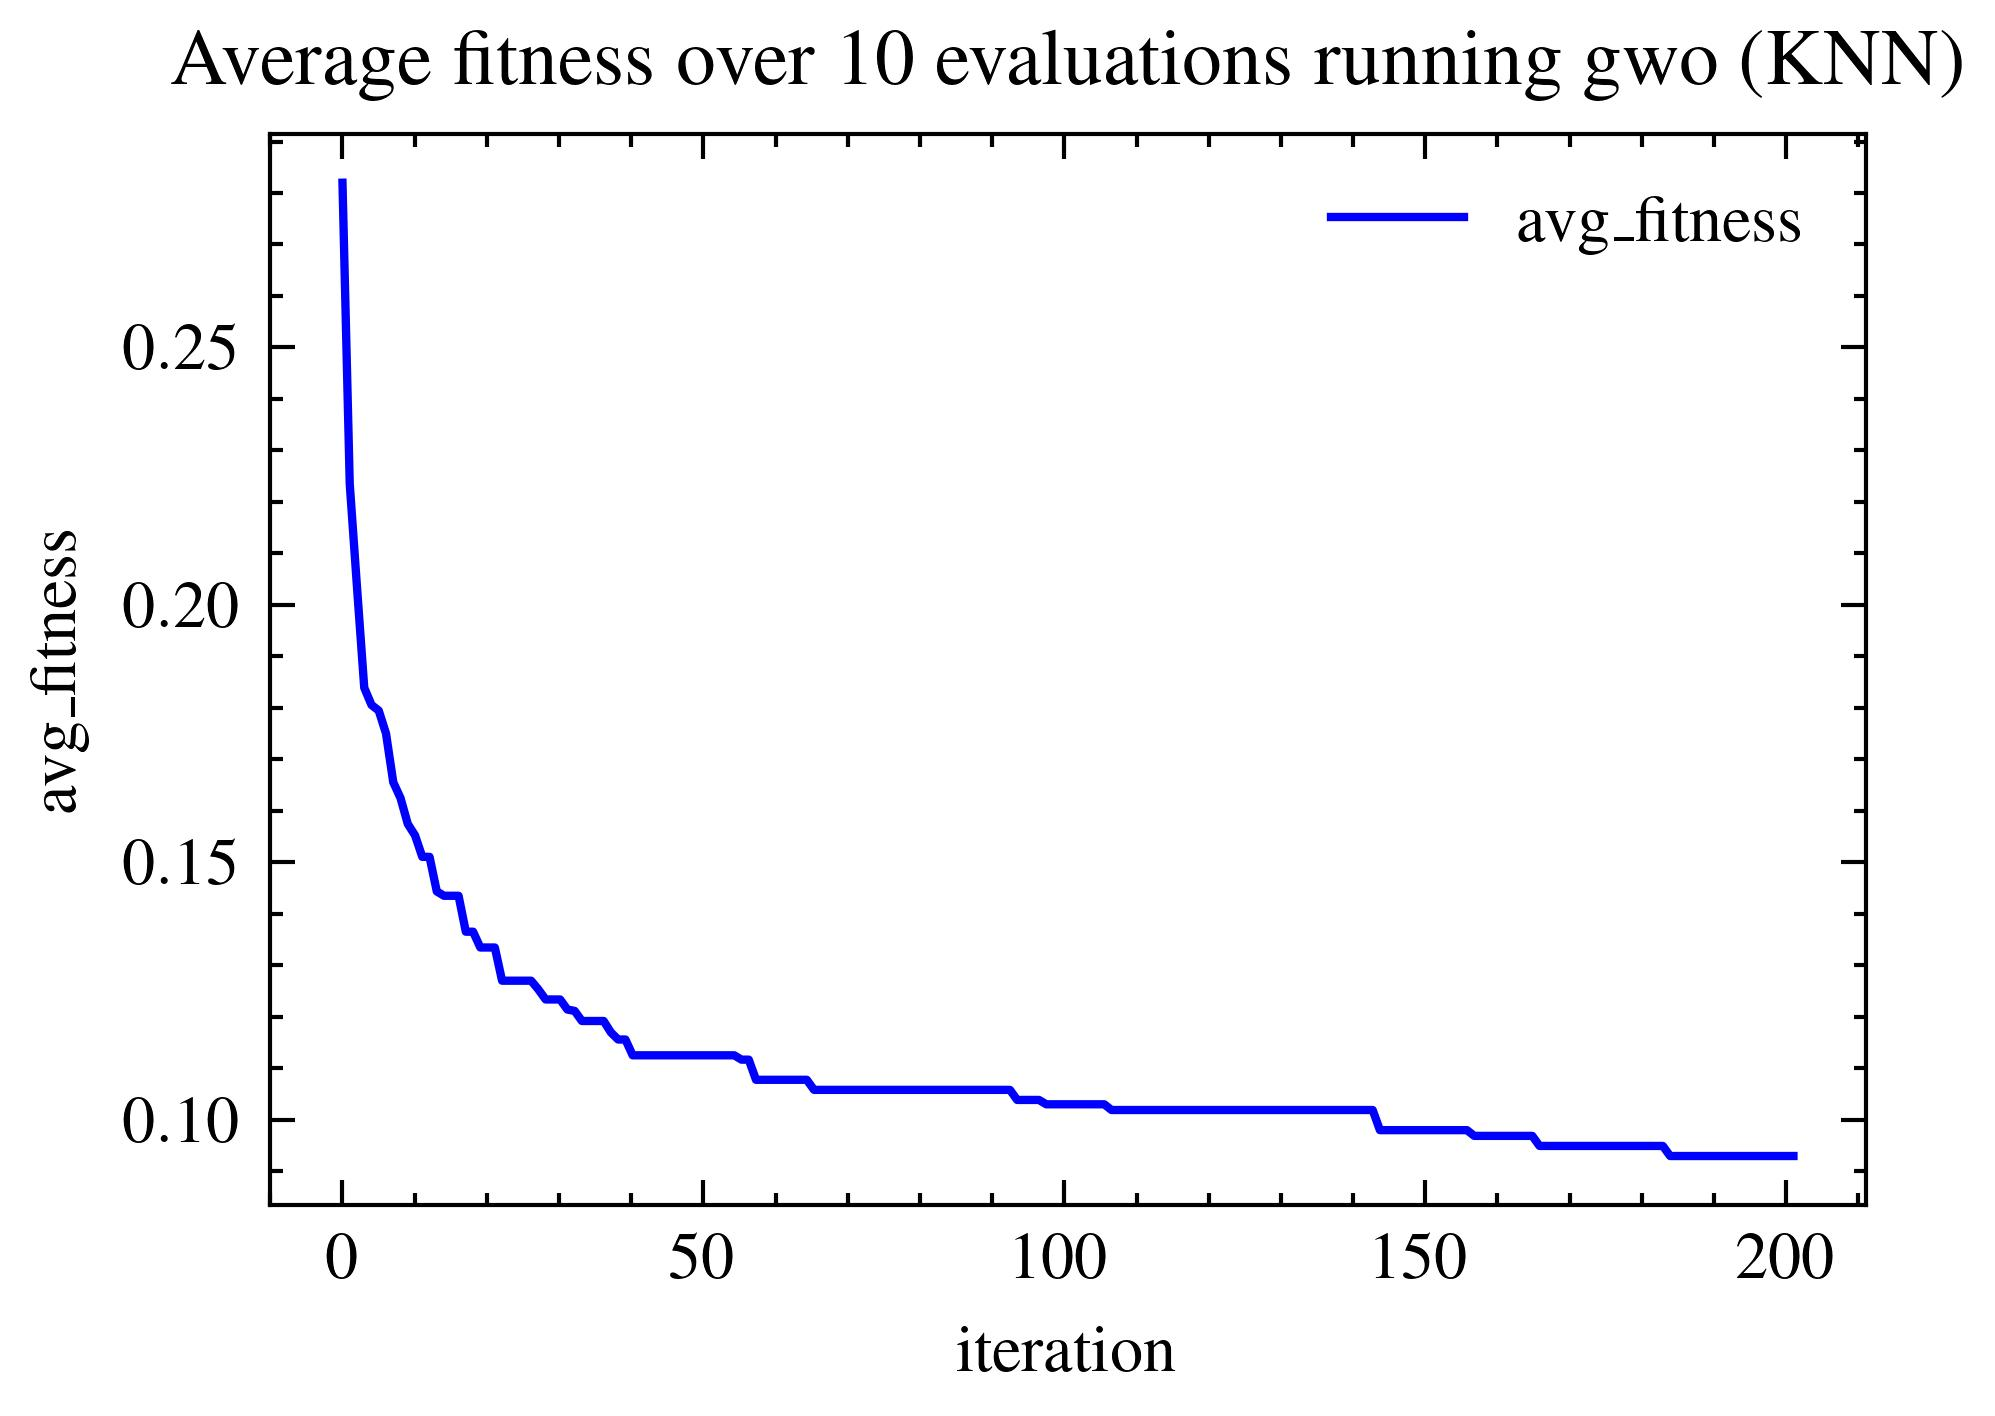
\includegraphics[width=\textwidth]{imagenes/binary_knn_fitness/KNN_fitness_over_10_evaluations_gwo_binary_breast-cancer.jpg}
        \caption{GWO}
        \label{fig:sub11}
    \end{subfigure}
    \hfill
    \begin{subfigure}[b]{0.3\textwidth}
        \centering
        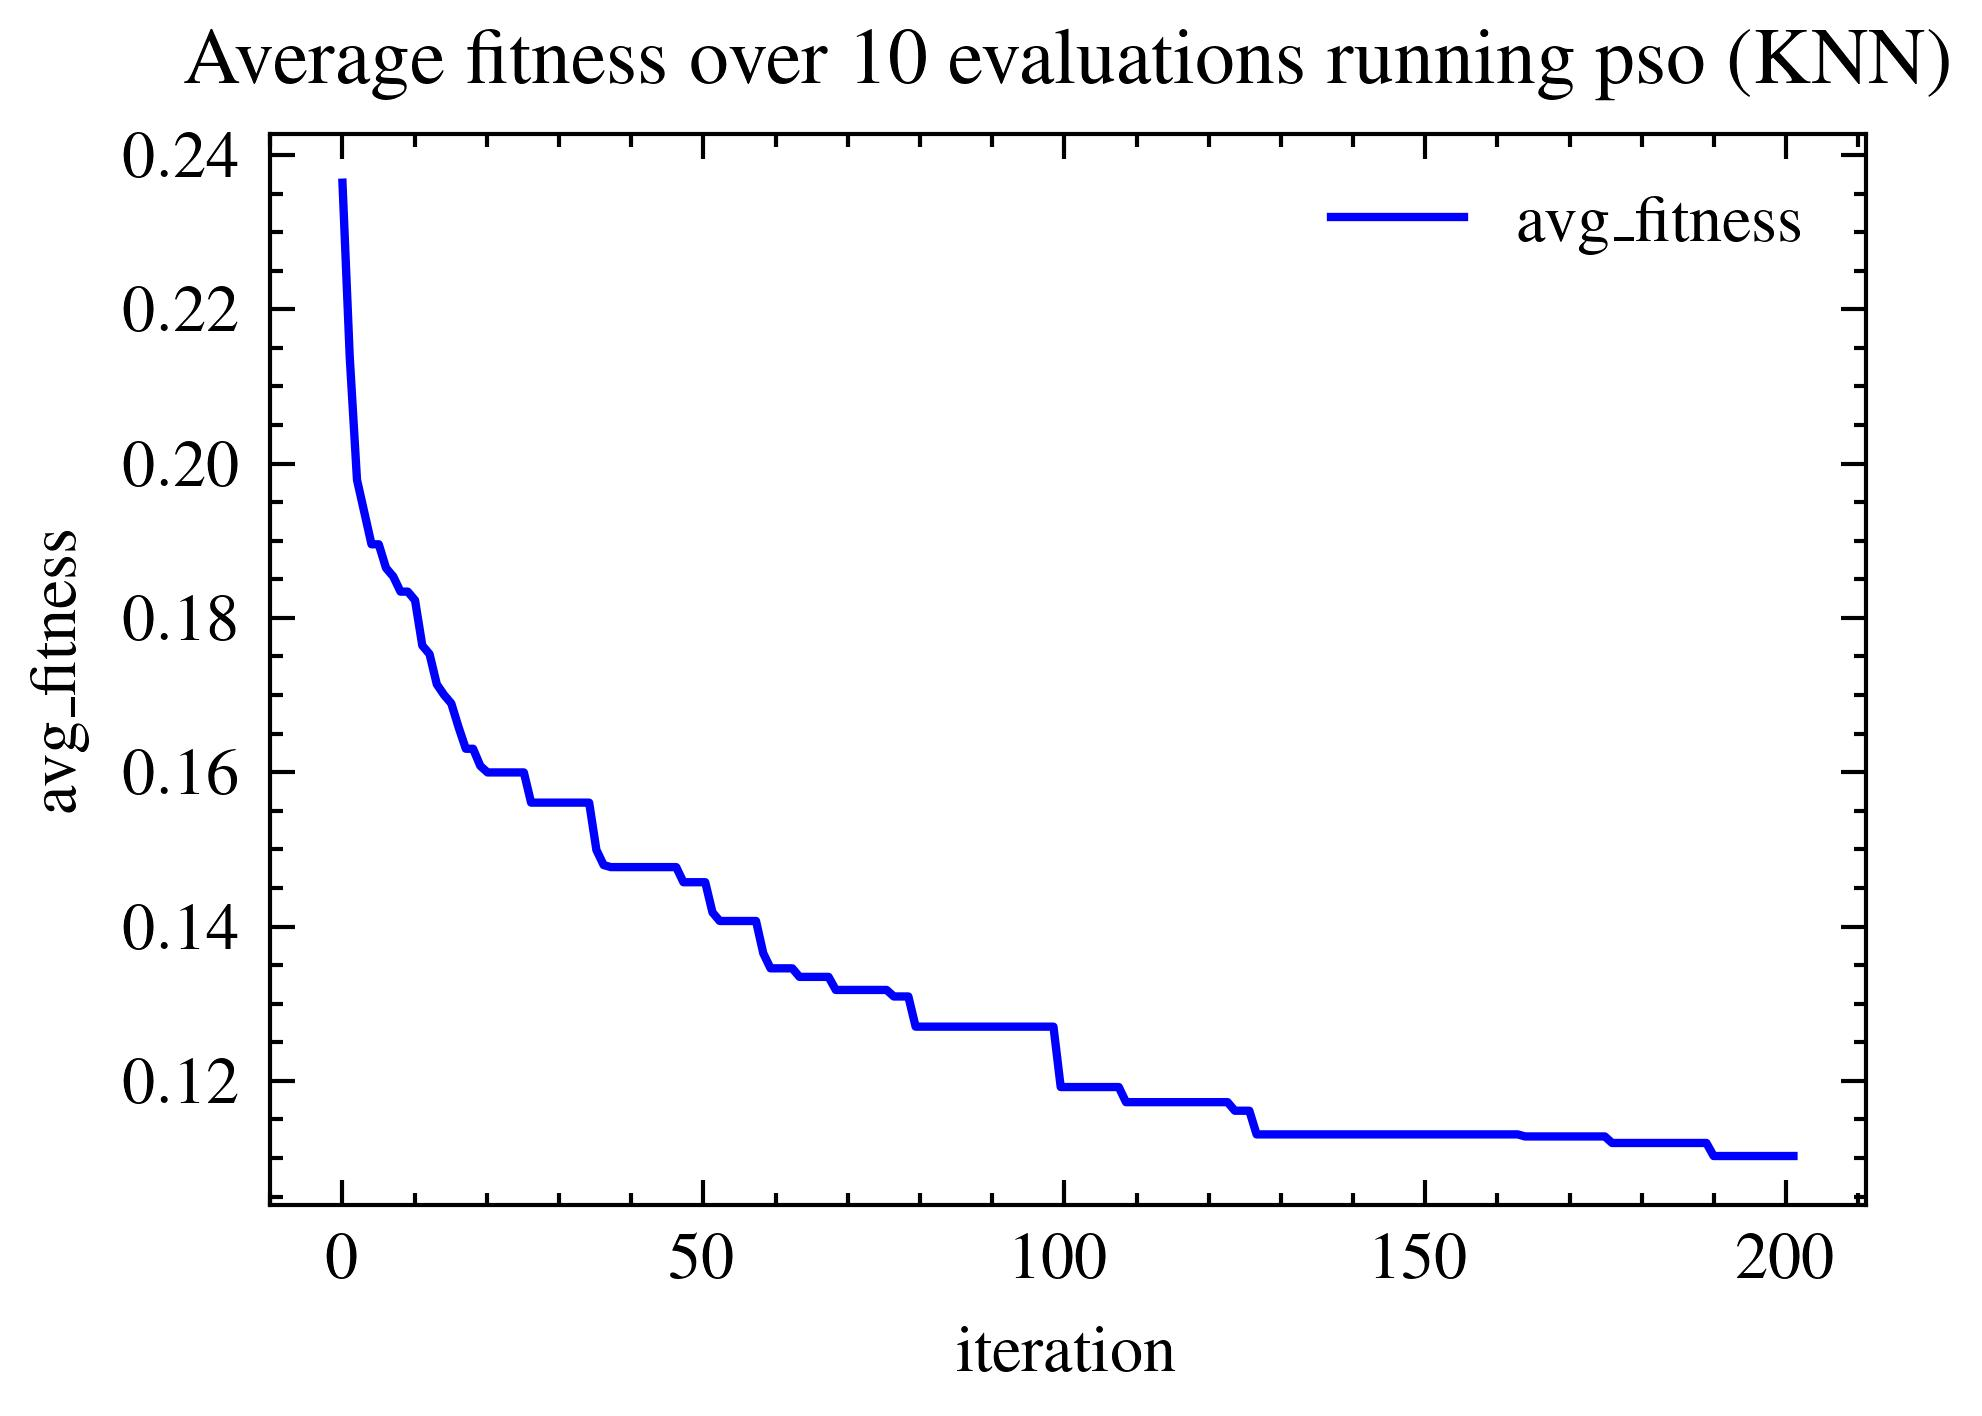
\includegraphics[width=\textwidth]{imagenes/binary_knn_fitness/KNN_fitness_over_10_evaluations_pso_binary_breast-cancer.jpg}
        \caption{PSO}
        \label{fig:sub12}
    \end{subfigure}
    
    \begin{subfigure}[b]{0.3\textwidth}
        \centering
        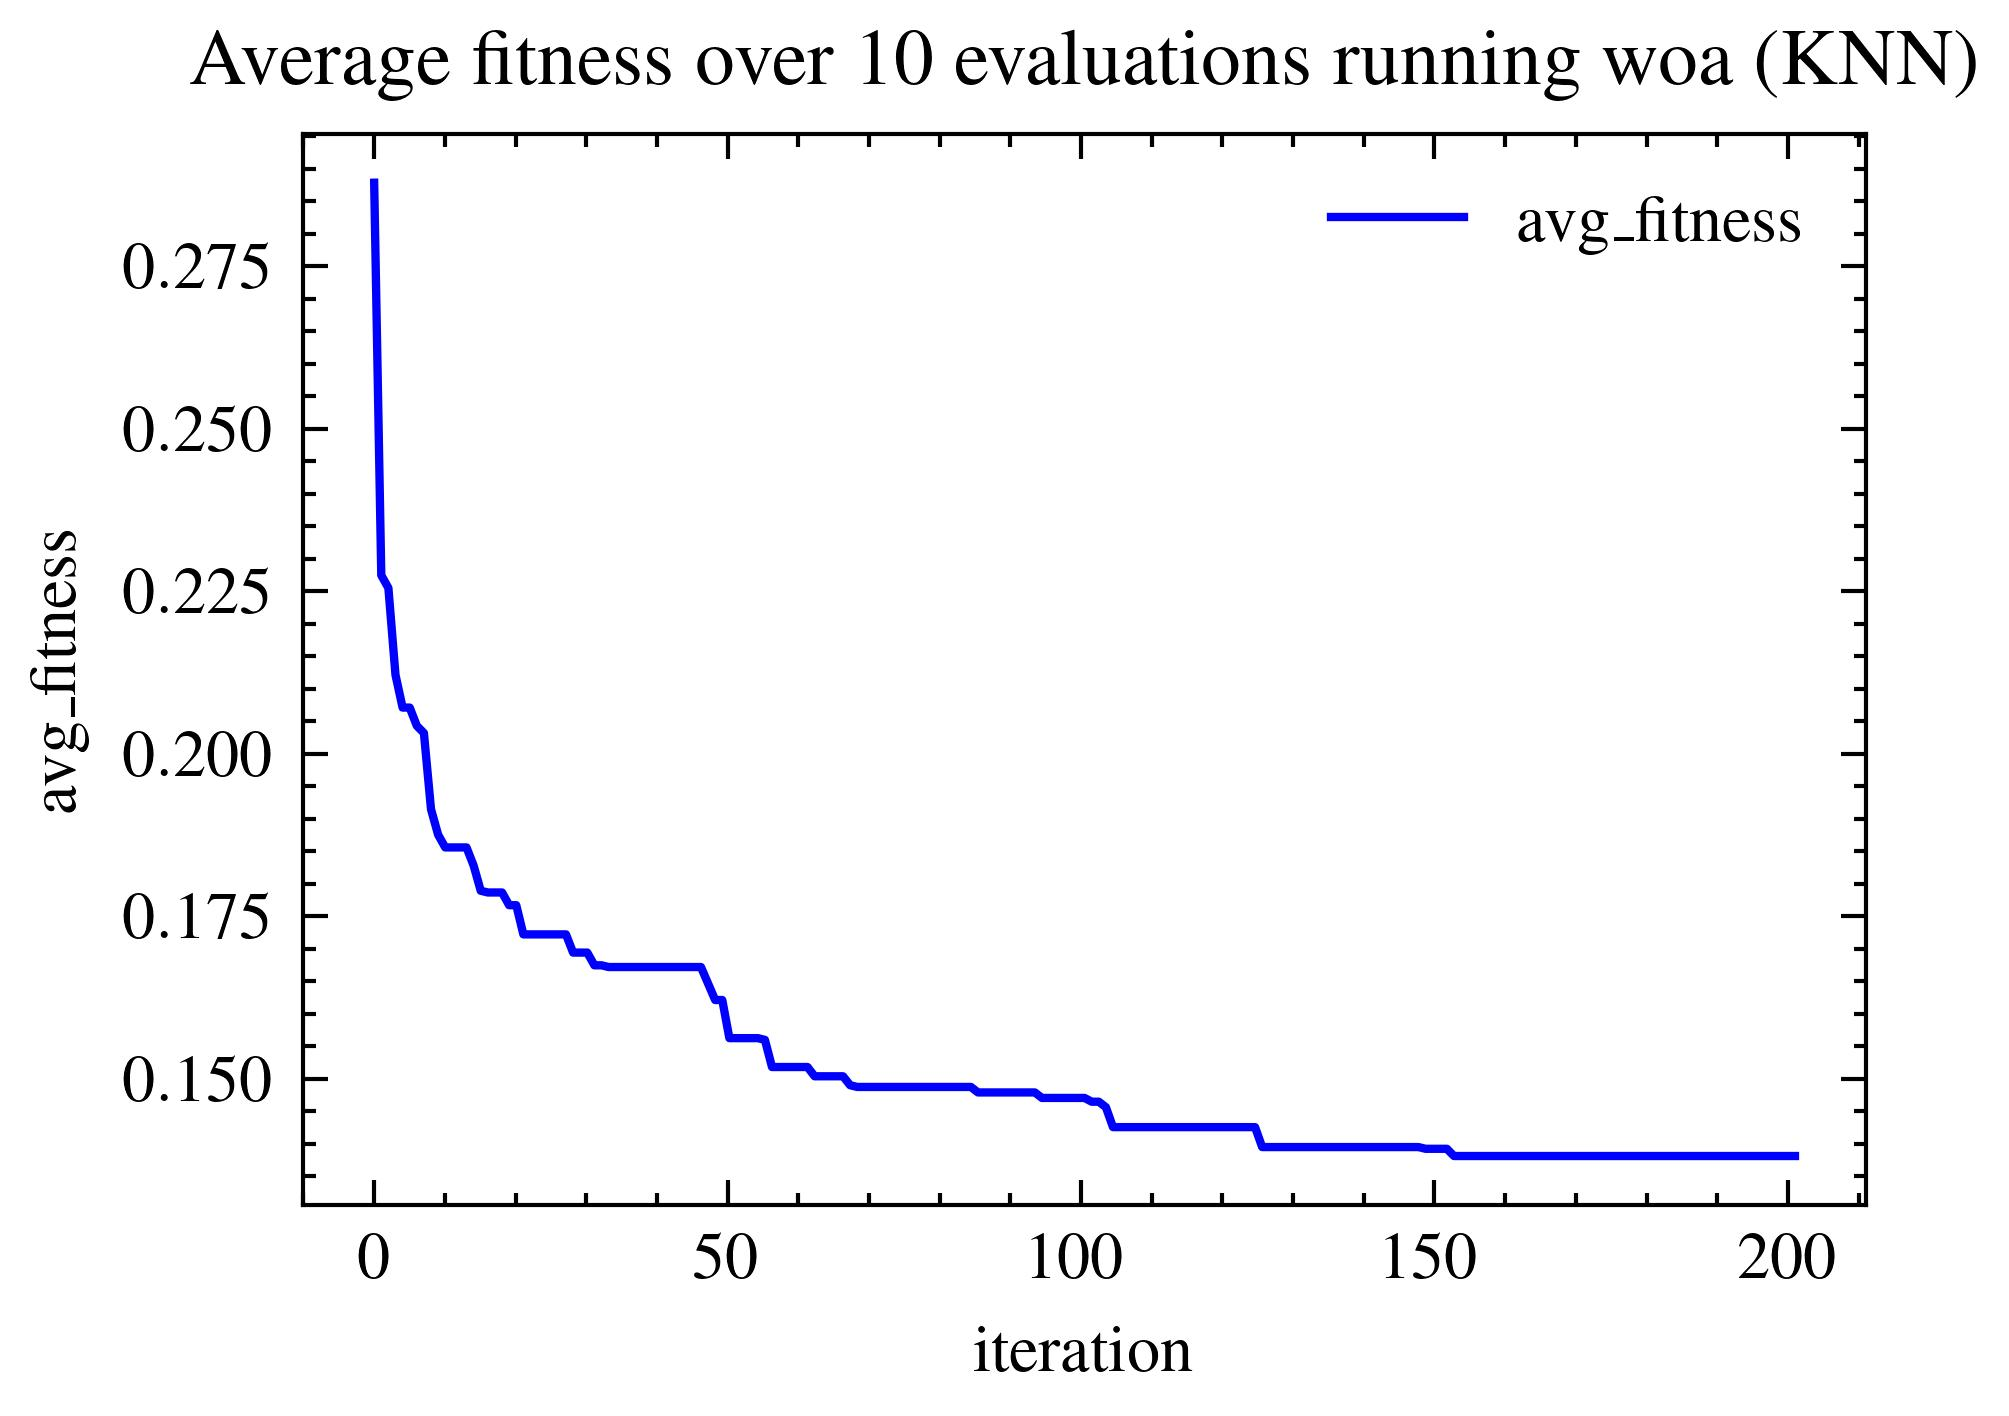
\includegraphics[width=\textwidth]{imagenes/binary_knn_fitness/KNN_fitness_over_10_evaluations_woa_binary_breast-cancer.jpg}
        \caption{WOA}
        \label{fig:sub13}
    \end{subfigure}

    \caption{Rendimiento durante 10 evaluaciones para varios algoritmos binarios en el conjunto de datos breast-cancer}
    \label{fig:all}
\end{figure}

\end{document}
